%%%%%%%%%%%%%%%%%%%%%%%%%%%%%%%%%%%%%%%%%%%%%%%%%%%%%%%%%%%%%%%%%%% 
%                                                                 %
%                         Capítulo 3                           %
%                                                                 %
%%%%%%%%%%%%%%%%%%%%%%%%%%%%%%%%%%%%%%%%%%%%%%%%%%%%%%%%%%%%%%%%%%% 

\chapter{Resultados}

\section{Descripción de la base}
  
La información sobre la cual se trabajó corresponde a la base de datos de CONAPO (Consejo Nacional de Población): ``Índice de Marginación por Entidad Federativa y Municipio 2010''. La base cuenta con $2,456$ observaciones y cada una tiene $15$ atributos descritos en la tabla \ref{descripvar} que corresponden a variables para medir el grado de marginación de un municipio.  

Para cada observación, se cuenta con un polígono geolocalizado que corresponde a la forma del municipio o delegación. Entonces, nuestra área de estudio espacial es la República Mexicana, que  corresponde a una retícula irregular, donde cada región corresponde a un municipio.

\begin{table}
\caption[Descripción de la base de datos]
            {Leyenda variables de marginación 2010.}
\label{descripvar}
\begin{tabular}{l p{10cm} r}
\hline
Variable & Descripción \\
\hline 
clave\_ent & Clave de la entidad federativa  \\	
clave\_mun & Clave de municipio	\\
nom\_mun	& Nombre del municipio \\
poblac & Población total \\
analf & \% de Población de 15 años o más analfabeta  \\ 
sprim & \%  de Población de 15 años o más sin primaria completa  \\ 
sdren  & \% Ocupantes en viviendas sin drenaje ni excusado  \\ 
selec & \% Ocupantes en viviendas sin energía eléctrica  \\ 
sagua & \% Ocupantes en viviendas sin agua entubada  \\ 
hacina & \% Viviendas con algún nivel de hacinamiento \\ 
pisot & \% Ocupantes en viviendas con piso de tierra  \\ 
pl5khab & \% Población en localidades con menos de 5 000 habitantes  \\ 
bingreso & \% Población ocupada con ingreso de hasta 2 salarios mínimos \\ 
imarg & Índice de marginación  \\ 
gmarg & Grado de marginación  \\ 
imarges & Índice de marginación escalado de 0 a 100  \\
lugar & Lugar que ocupa a nivel nacional \\
\hline 
\end{tabular} 
\end{table}

Las variables analf, sprim, sdren, selec, sagua, hacina, pisot, l5kha y bingreso son indicadores de marginación definidos por \citet{conapo04} (Consejo Nacional de Población) que miden el nivel de marginación en cuatro dimensiones: educación, vivienda, distribución de la población e ingresos monetarios. 

El valor del índice de marginación es la primera componente del método de componentes principales, aplicado a los nueve indicadores mencionados; una vez determinados los
valores para cada área, se clasifican en cinco grupos diferenciados y delimitados mediante la técnica de estratificación óptima de Dalenius y Hodges \citep{conapo11}.

\section{Análisis Exploratorio}


Empezamos observando el diagrama de dispersión  de Moran \ref{obj:moranplot} que compara el índice de marginación de un municipio contra el promedio de índice de marginación de sus vecinos, podemos observar que hay una correlación positiva muy alta. Esto es un síntoma de autocorrelación espacial positiva, pues esperamos valores parecidos de índice de marginación entre vecinos. 

Los puntos que están por arriba de la nube de puntos tienen menor índice de marginación con respecto a sus vecinos; en contraste, puntos por debajo de la nube, tienen mayor índice de marginación con respecto a sus vecinos.

Se realizó una regresión lineal simple para encontrar aquellas observaciones cuyos residuales son altos. 

\begin{figure}[!ht]
\centering
% 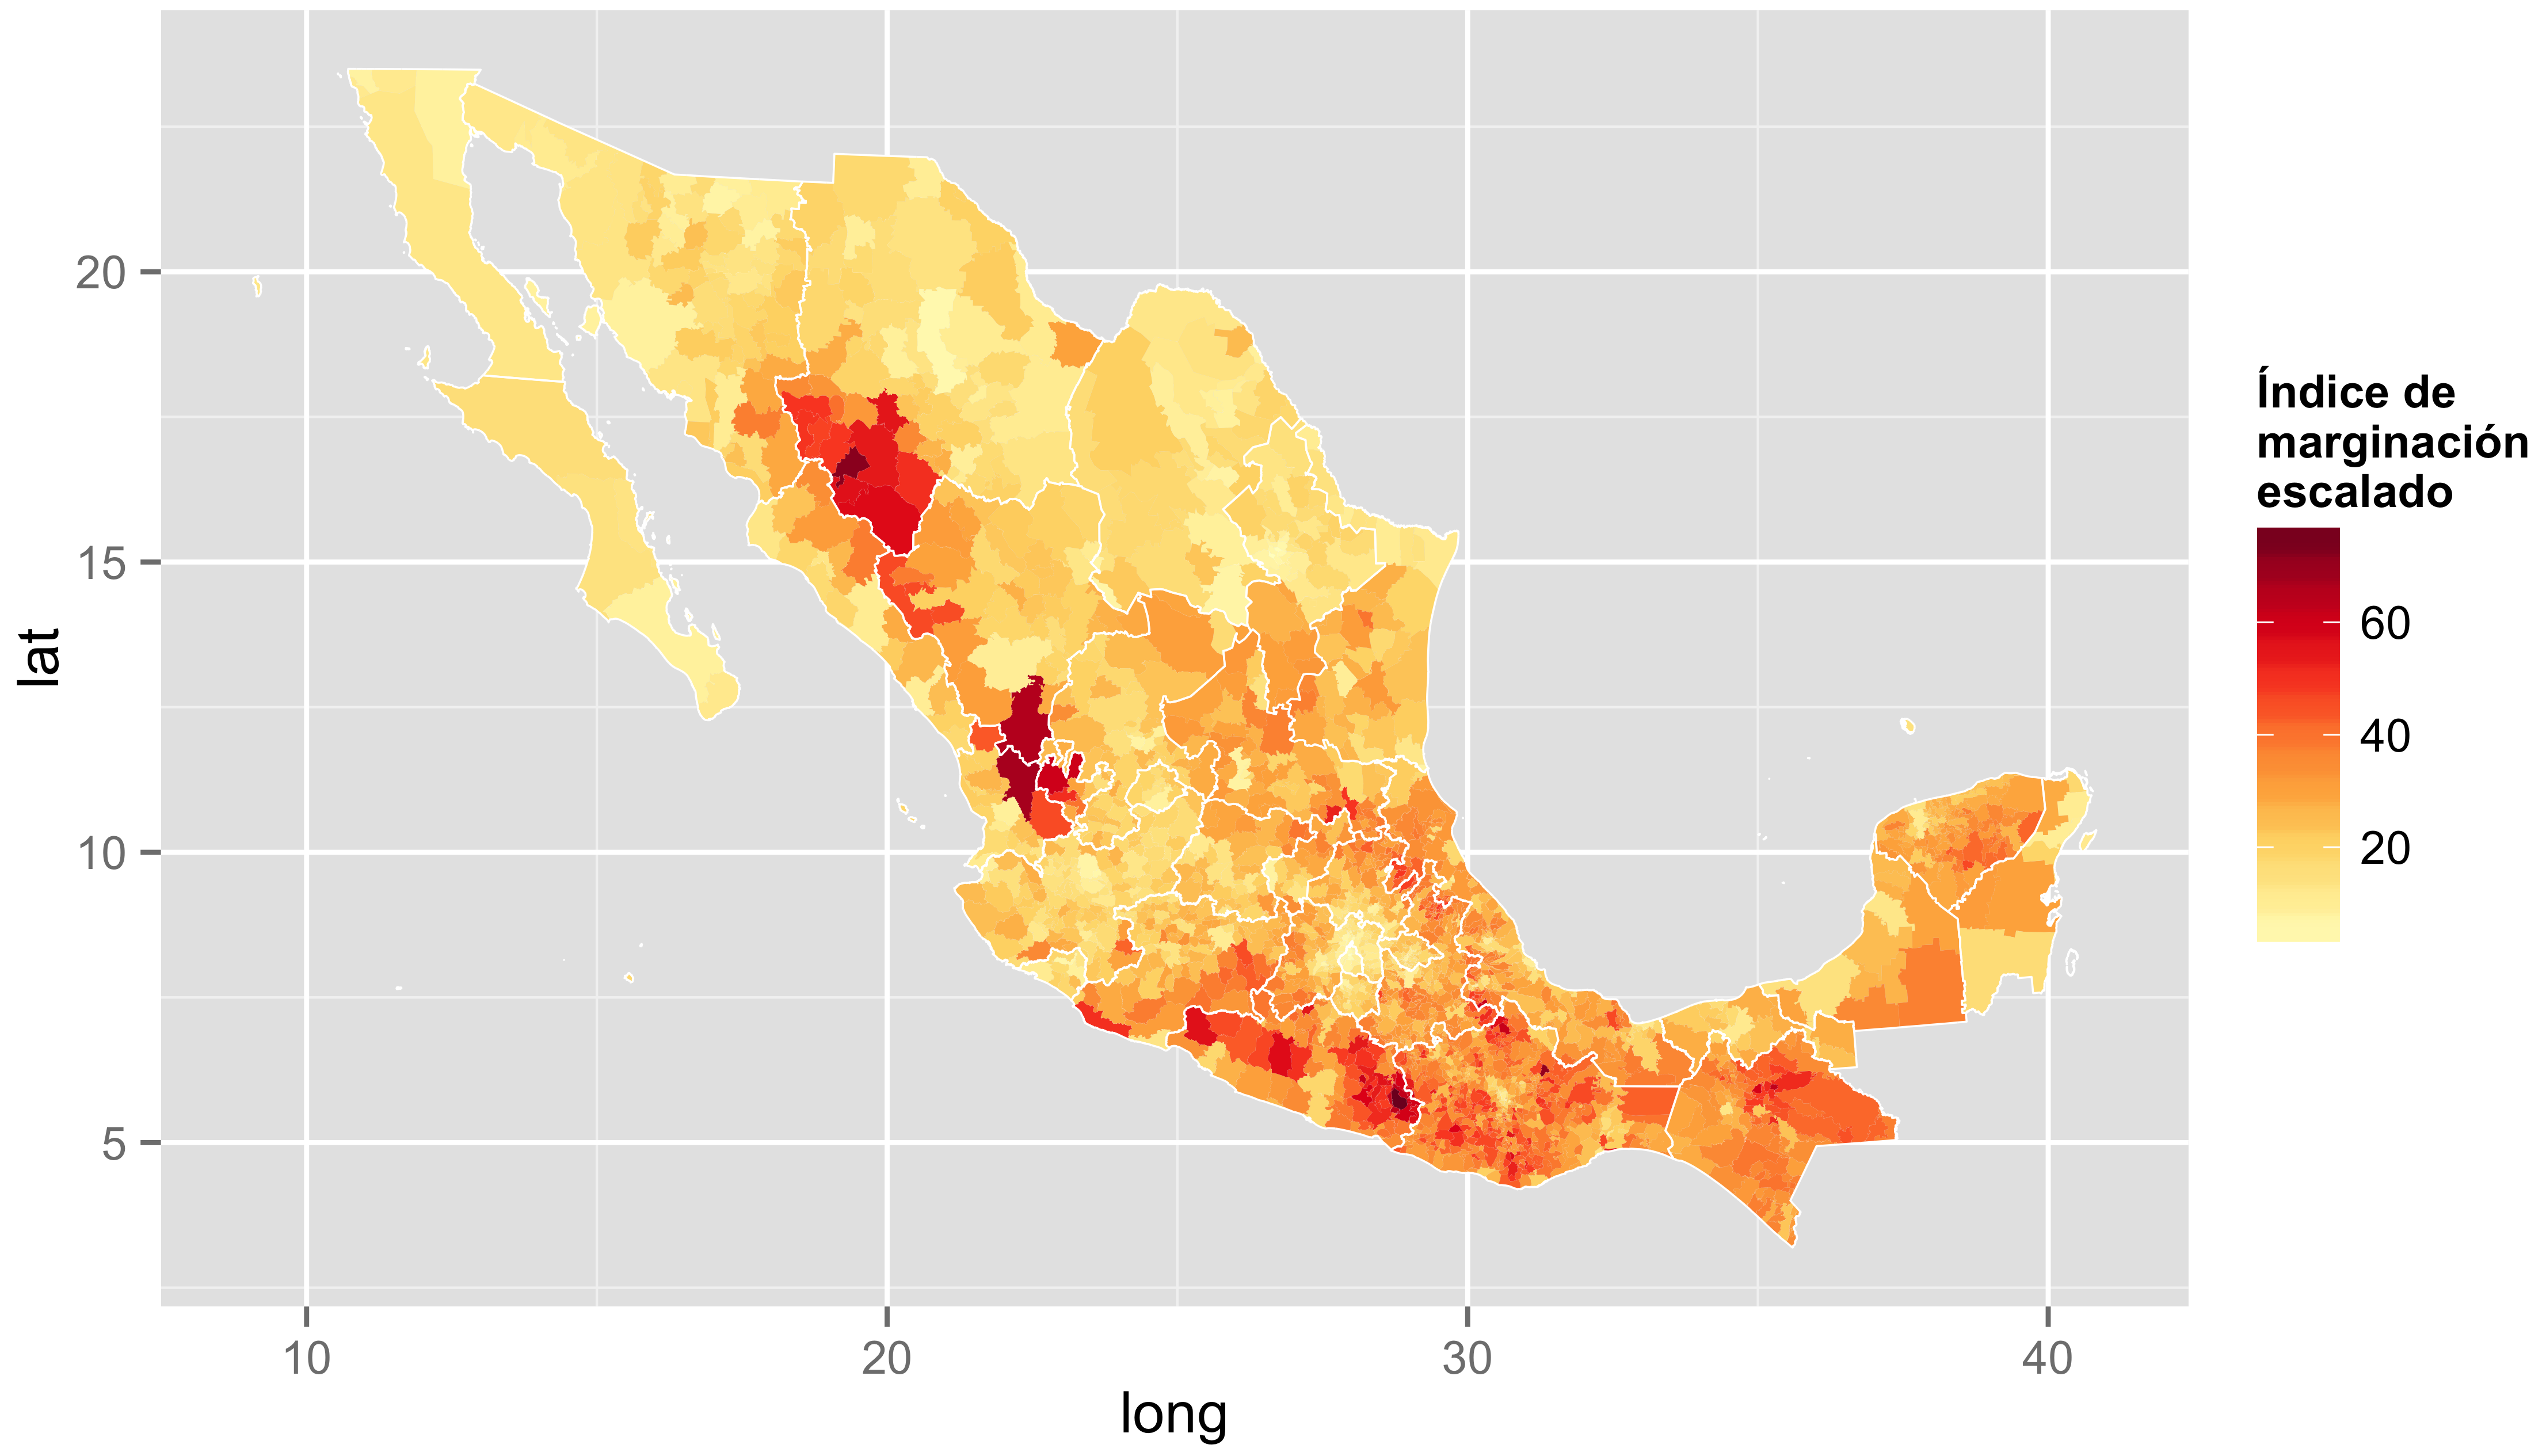
\includegraphics[scale=.20]{./maps/mapmarg.png} \\
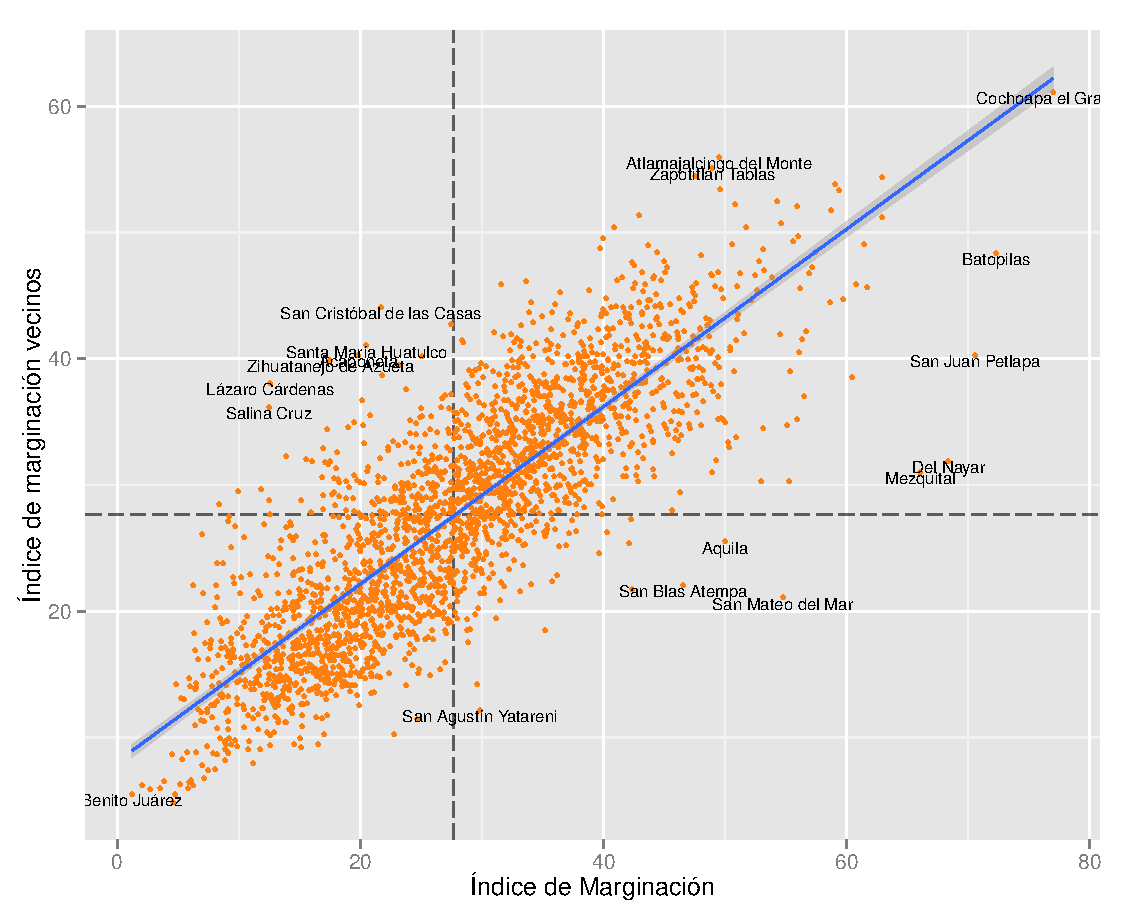
\includegraphics[width=.95\textwidth]{./plots/moran_plot.pdf} \\
\caption{Gráfica de Moran para índice de marginación.}
\label{obj:moranplot}  
\end{figure}

Algunos casos interesantes son los siguientes:
\begin{itemize}
\item Podemos ver que San Mateo del Mar está muy lejos y por debajo de la nube de puntos, su índice de marginación es muy alto en comparación con el de sus vecinos. En contraste, vemos en la parte de arriba a la izquierda al municipio de Salina Cruz, que tiene un índice de marginación más bajo. De hecho, ambos municipios son vecinos en el estado de Oaxaca. Salina Cruz es un importante centro industrial, debido a la presencia de la Refinería Ing. Antonio Dovalí Jaime de PEMEX.

\item Otros municipios que se encuentran muy por debajo de la curva, son Mezquital, en Durango y Del Nayar, en Nayarit. Estos municipios ocupan el quinto y el tercer lugar de marginación a nivel nacional respectivamente. Aunque estén en estados diferentes, ambos municipios comparten frontera y por lo tanto, tienes características similares. Los dos son municipios que se mantuvieron al margen de la evolución ocurrida en el resto de su entidad correspondiente, por la concentración de población indígena. Ambos ocupan el primer lugar de marginación dentro de su entidad. Se pueden apreciar en el mapa ~\ref{obj:mapmarg} de color rojo intenso, al sur de Durango y norte de Nayarit.

\item En el caso de San Cristobal de las Casas, está por arriba de la nube de puntos. Es el municipio de Chiapas con menor índice de marginación. Esto se puede deber al turismo y a las inversiones en la región. 
\end{itemize}

El mapa coroplético \ref{obj:mapmarg} muestra de manera clara que hay una alta autocorrelación espacial positiva en el índice de marginación. Se puede observar que en general hay una transición suave entre colores obscuros y claros, es decir, entre municipios vecinos hay colores muy parecidos, lo que indica valores de marginación cercanos.  

Encontramos puntos rojos obscuros de alta marginación en lugares como la Sierra Tarahumara al suroeste de Chihuahua, sur de Durango y norte de Nayarit (Mezquital y Del Nayar), límites entre Puebla y Veracruz,  los estados de Oaxaca, Guerrero y Chiapas, etc.

\begin{landscape}
\begin{figure}[!ht]
\centering
% 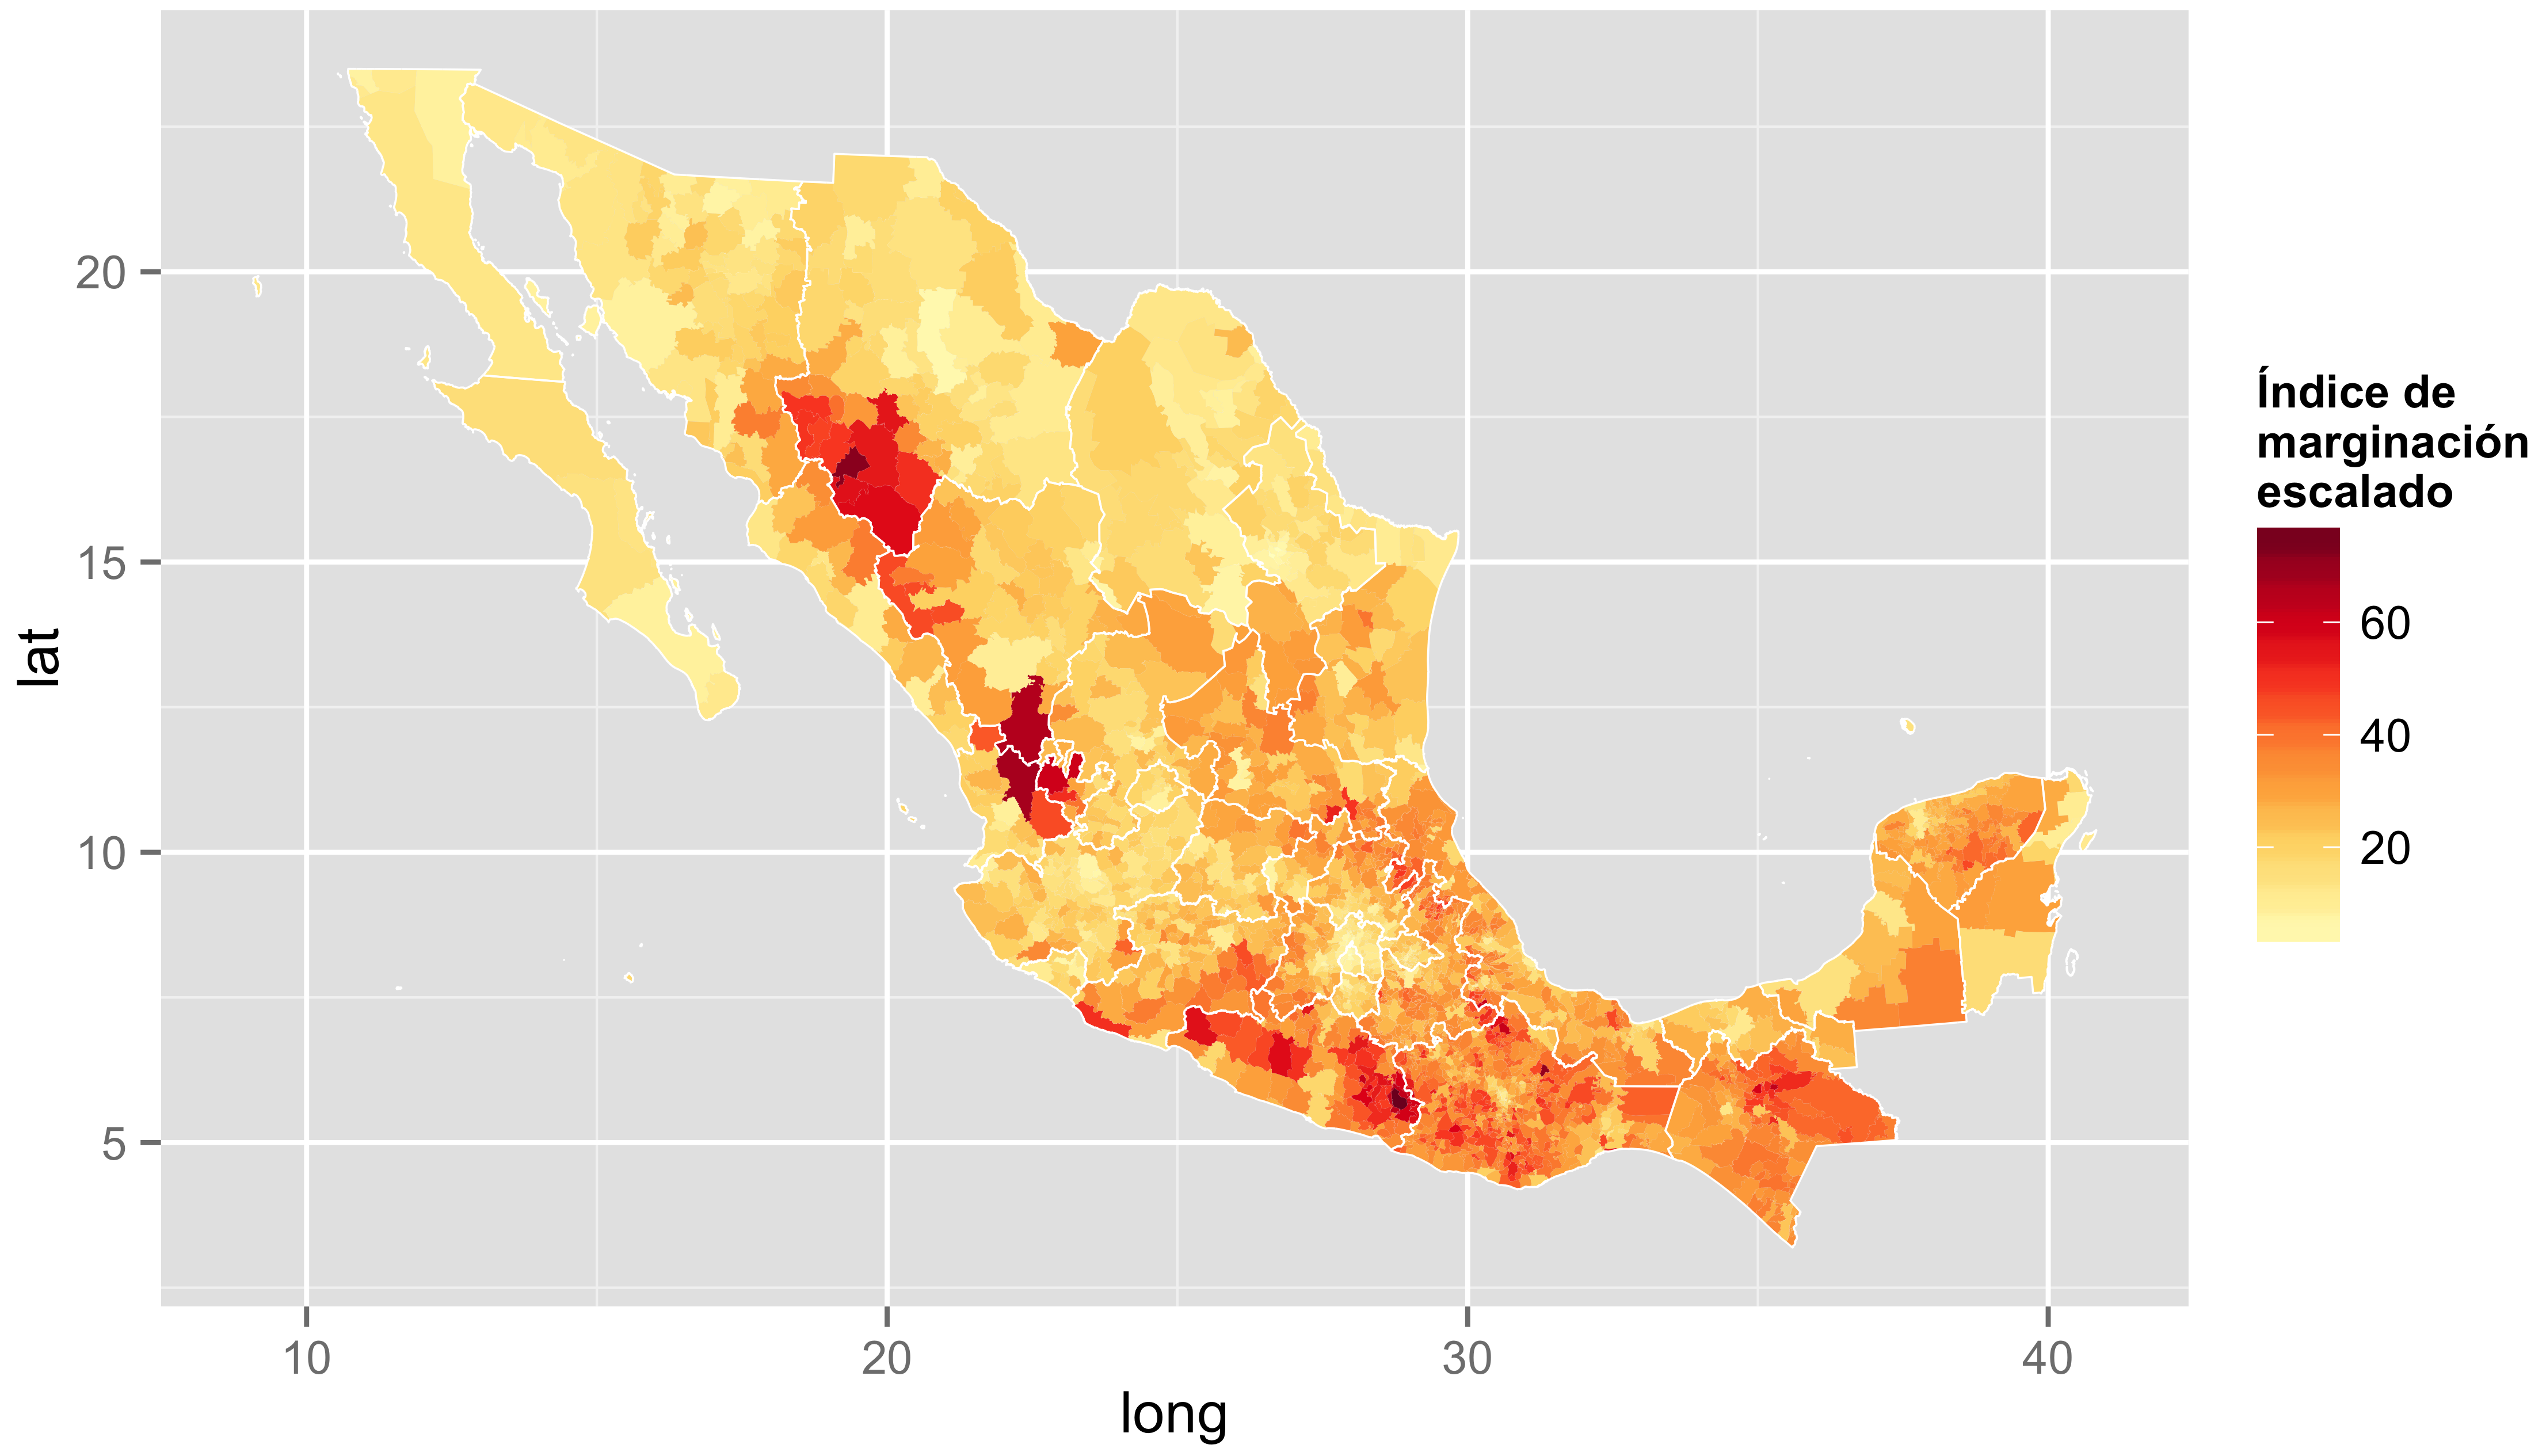
\includegraphics[scale=.20]{./maps/mapmarg.png} \\
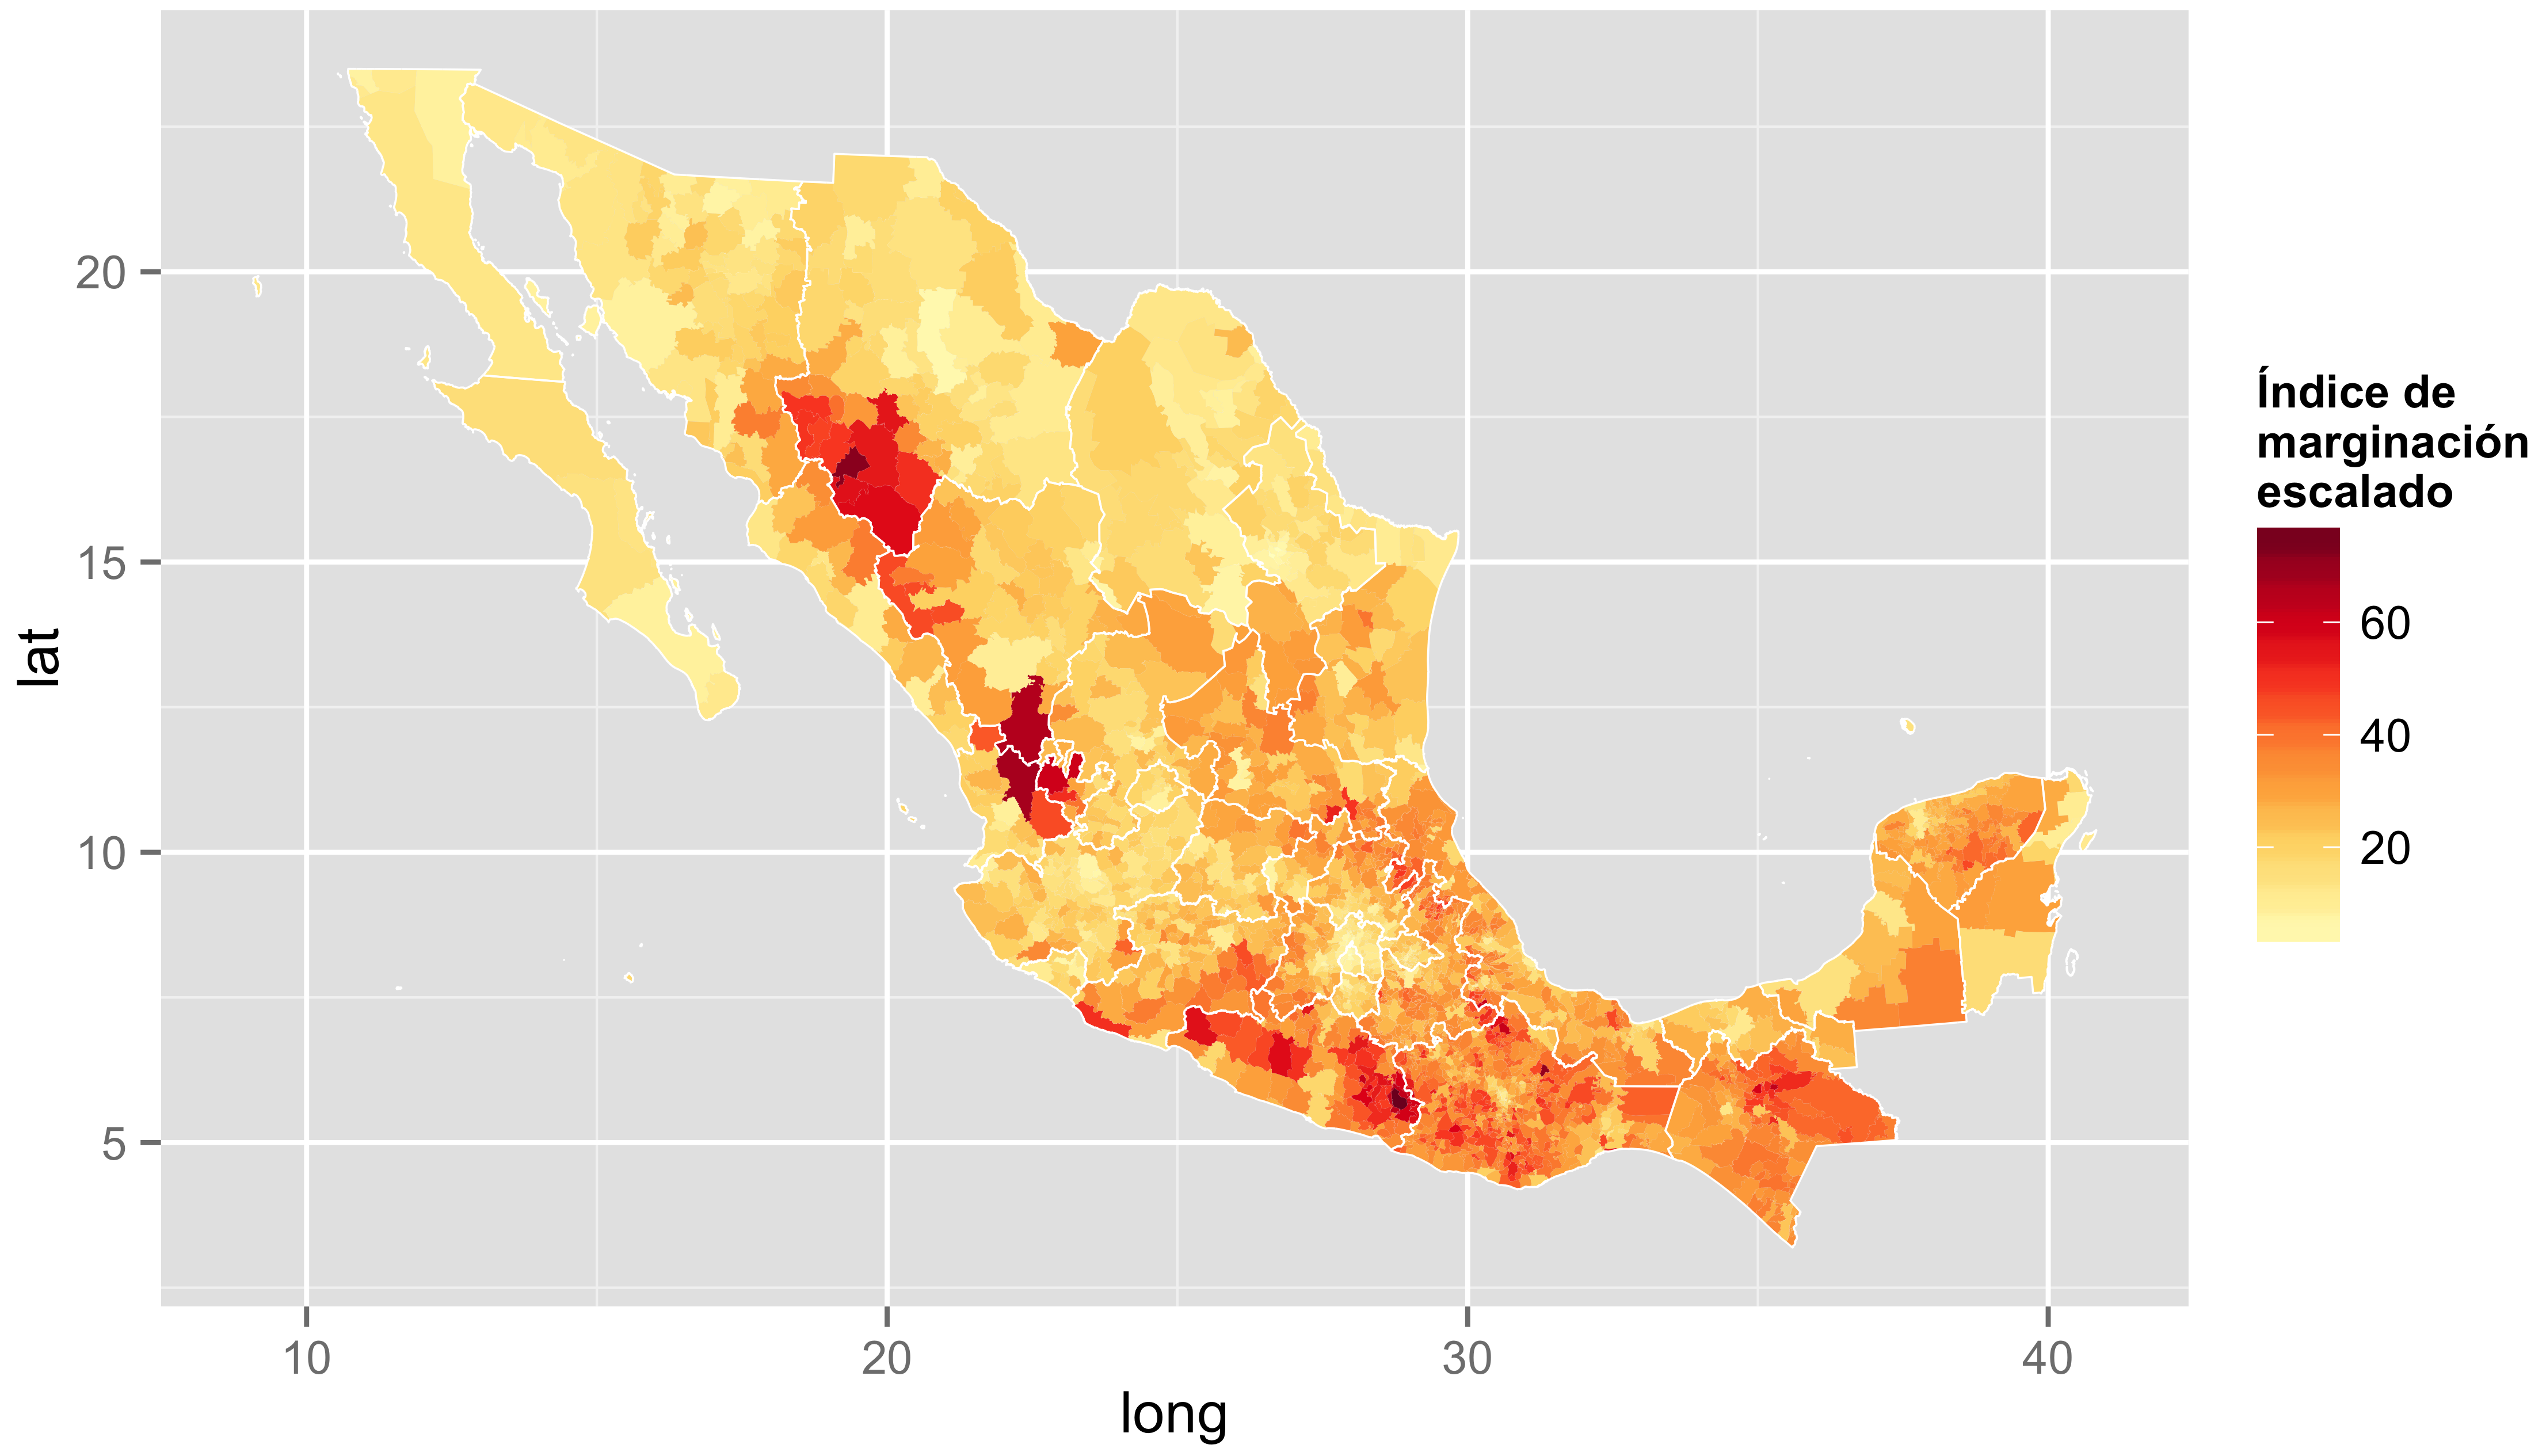
\includegraphics[width=1.4\textheight]{./maps/mapmarg.png} \\
\caption{Mapa de México coloreando cada municipio por su índice de marginación.}
\label{obj:mapmarg}  
\end{figure}
\end{landscape}

Las tabla \ref{tab:masmarg}  muestra los municipios más marginados. Aparecen los casos de Mezquital y Del Nayar mencionados anteriormente. Batopilas es un municipio que se encuentra en la Sierra Tarahumara en Chihuahua; San Juan Petlapa, en Oaxaca y  Cochoapa el Grande, el municipio más marginado, en Guerrero.

\begin{table}[ht]
\centering
\begin{tabular}{llrl}
  \hline
nom\_mun & gmarg & imarges & lugar \\ 
  \hline
  Cochoapa el Grande & Muy alto & 76.98 & 1 \\
  Batopilas & Muy alto & 72.27 & 2 \\ 
  San Juan Petlapa & Muy alto & 70.55 & 3 \\ 
  Del Nayar & Muy alto & 68.38 & 4 \\
  Mezquital & Muy alto & 66.06 & 5 \\ 
   \hline
\end{tabular}
\caption[Municipios más marginados]
            {Tabla de municipios más marginados,}
\label{tab:masmarg}
\end{table}



La lista de los municipios menos marginados se encuentra en la tabla \ref{tab:menosmarg}. Destacan tres delegaciones del Distrito Federal (Coyoacán, Miguel Hidalgo y Benito Juárez)  y dos municipios que forman parte de la zona metropolitana de la Ciudad de Monterrey en Nuevo León (San Pedro Garza García y San Nicolás de los Garza).

\begin{table}[ht]
\centering
\begin{tabular}{llrl}
  \hline
nom\_mun & gmarg & imarges & lugar \\ 
  \hline
  Coyoacán & Muy bajo & 3.86 & 2,452 \\ 
  Miguel Hidalgo & Muy bajo & 3.56 & 2,453 \\   
  San Nicolás de los Garza & Muy bajo & 2.69 & 2,454 \\ 
  San Pedro Garza García & Muy bajo & 2.09 & 2,455 \\
  Benito Juárez & Muy bajo & 1.21 & 2,456 \\ 
  \hline
\end{tabular}
\caption[Municipios menos marginados]
            {Tabla de municipios menos marginados.}
\label{tab:menosmarg}
\end{table}

En la gráfica~\ref{obj:gradosmarg} se presenta el conteo de municipios por nivel de grado de marginación por estado.

\begin{figure}[!ht]
\centering
% 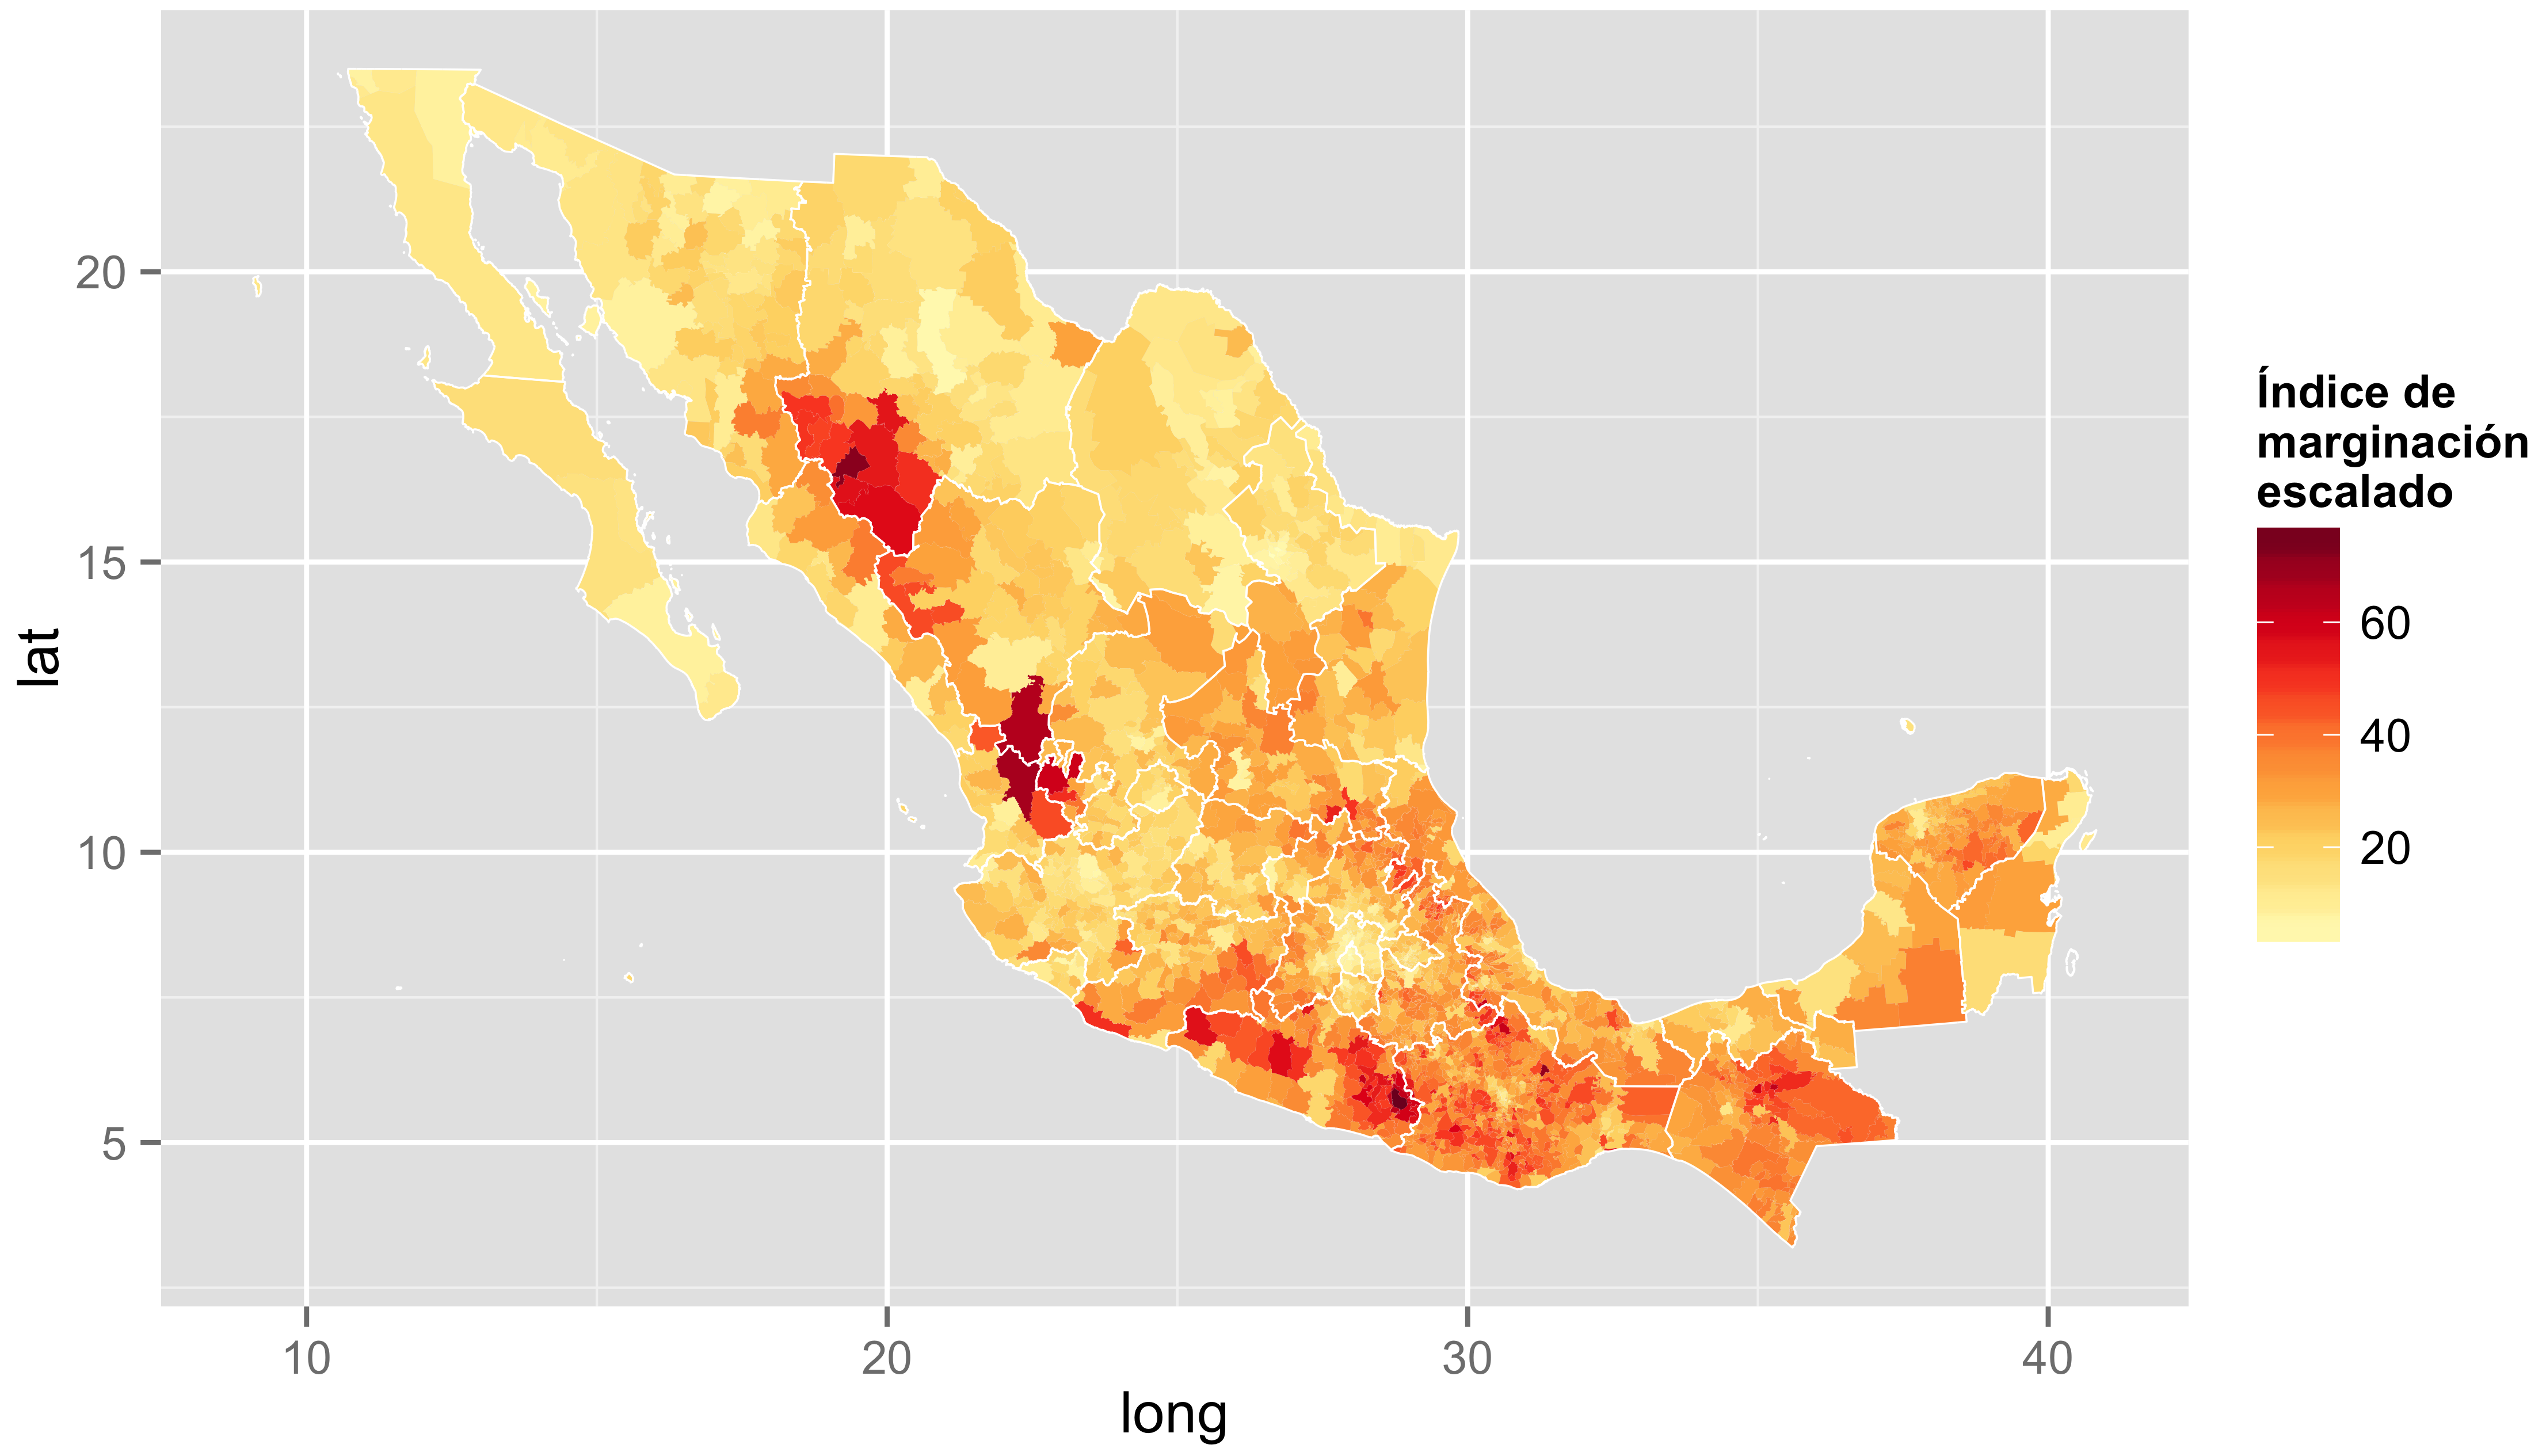
\includegraphics[scale=.20]{./maps/mapmarg.png} \\
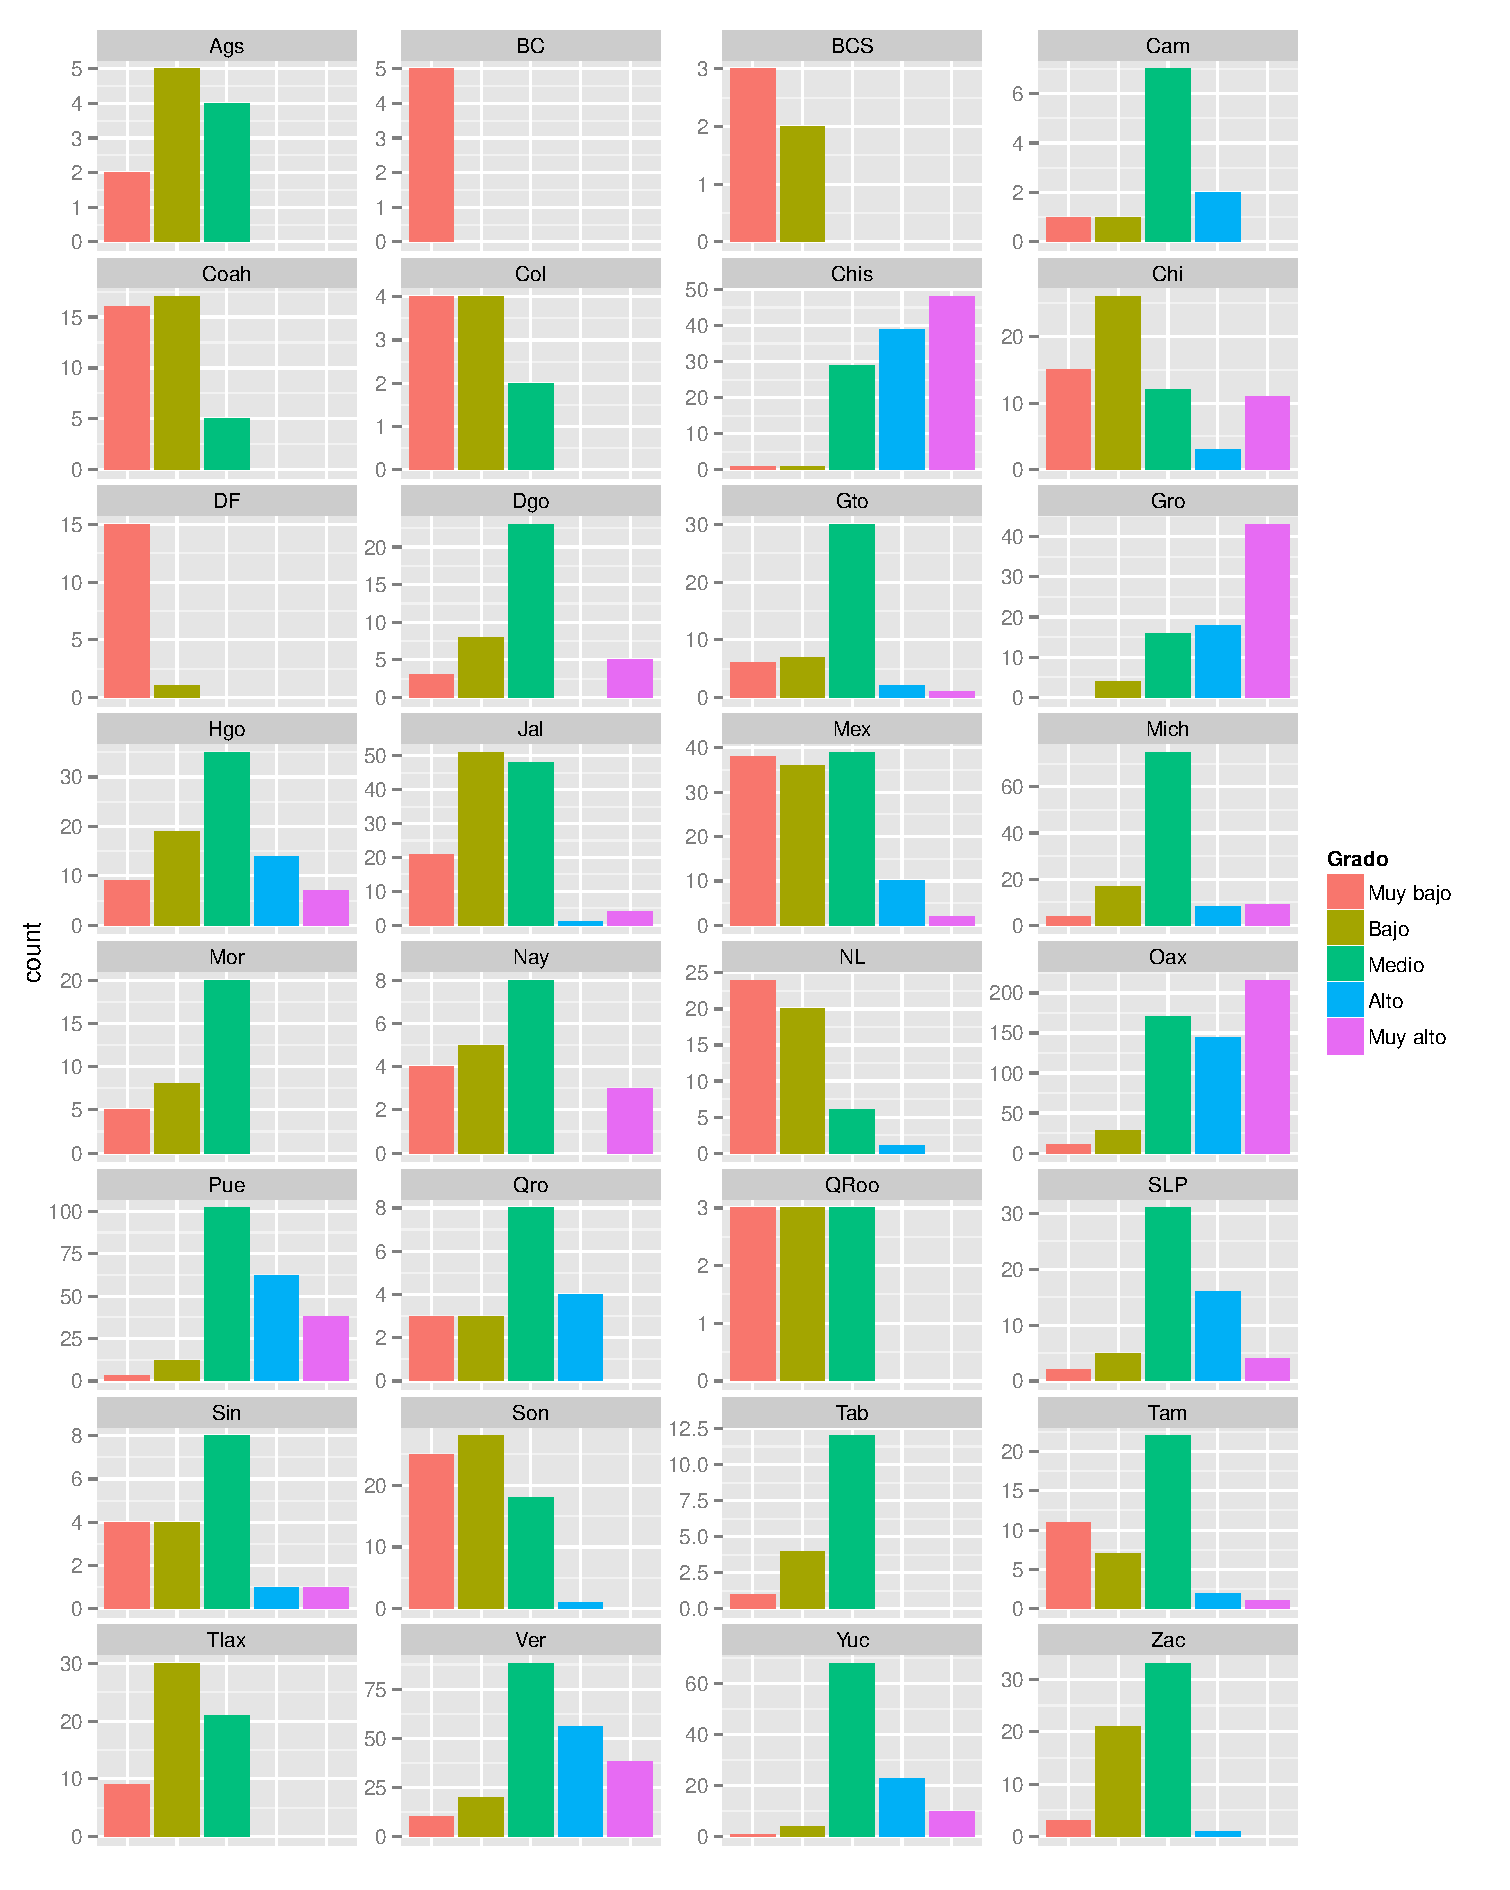
\includegraphics[width=\textwidth]{./plots/gmarg_plot.pdf} \\
\caption{Conteo grados de marginación.}
\label{obj:gradosmarg}  
\end{figure}

Observamos que Guerrero, Chiapas y Oaxaca destacan por tener gran proporción de municipios con grados de marginación ``Alto'' y ``Muy Alto'', corroborando lo que habíamos notado anteriormente con base en el mapa~\ref{obj:mapmarg}.

\section{Pruebas de autocorrelación espacial para índice de marginación}
Habiendo observado los datos, se harán las pruebas de autocorrelación espacial de Moran y de Geary para el índice de marginación.

Los pesos $w_{ij}$ a utilizar son los pesos binarios estandarizados por fila.
\subsection{Índice $\mathcal{I}$}
El valor del estimador $\mathcal{I}$, tiene el valor de 
\begin{equation}
\Hat{\mathcal{I}} = 0.703 .
\end{equation}

Sea $\mathcal{I}_0$ el valor esperado de $\mathcal{I}$ bajo la hipótesis nula, como esperamos autocorrelación espacial positiva para el índice de marginación, usamos la hipótesis alternativa $H_0: \mathcal{I}>\mathcal{I}_0$.


Utilizando los distintos supuestos, obtenemos los siguientes resultados.
\subsubsection{Bajo el supuesto de normalidad}
Se obtuvieron los siguientes resultados
\begin{align*}
\EN [ \widehat{\mathcal{I}}] =& -0.000407332,  \\ 
\VarN(\widehat{\mathcal{I}}) =& 0.000148633, \\
z =& 57.6945, \\
\mbox{valor-p} <& 2.2 \times 10^{-16}.
\end{align*}

El valor del estadístico $z$ está muy lejos de la región de no rechazo de $H_0$, es claro que rechazamos la hipótesis nula de no autocorrelación, y por lo tanto, $\Hat{\mathcal{I}}$ es significativamente mayor que $\mathcal{I}_0$.

\subsubsection{Bajo el supuesto de aleatorización}
Bajo el supuesto de aleatorización, se obtuvieron resultados bastante similares

\begin{align*}
\widehat{\ER [ \widehat{\mathcal{I}}]} =& -0.0004073320,  \\ 
\widehat{\VarN(\widehat{\mathcal{I}})} =& 0.0001486393, \\
z =& 57.6933, \\
\mbox{valor-p} <& 2.2 \times 10^{-16}.
\end{align*}

El valor del estadístico $z$ bajo este supuesto es practicamente el mismo que bajo el supuesto de normalidad, de la misma manera rechazamos la hipótesis nula de no autocorrelación espacial.
\subsubsection{Simulaciones de Monte Carlo}
Como el supuesto de normalidad es sensible es sensible a varios factores, es recomendable hacer simulaciones de Monte Carlo (vease \ref{sec:montecarlo}) para muestrear de la distribución de $\mathcal{I}$ .

Usando $n_{sim}=9999$, se obtuvieron los siguientes resultados
\begin{align*}
\mbox{orden observado} =& 10000,\\
\mbox{valor-p} =& 1\times 10^{-4}.
\end{align*}

Es decir, las  $9999$ observaciones del muestreo cayeron por debajo de $\Hat{\mathcal{I}}$. Por lo tanto, esta prueba también nos indica claramente autocorrelación espacial positiva.

En la gráfica \ref{obj:morandensity} podemos ver la densidad obtenida a partir de la muestra de Monte Carlo. 

\begin{figure}[!ht]
\centering
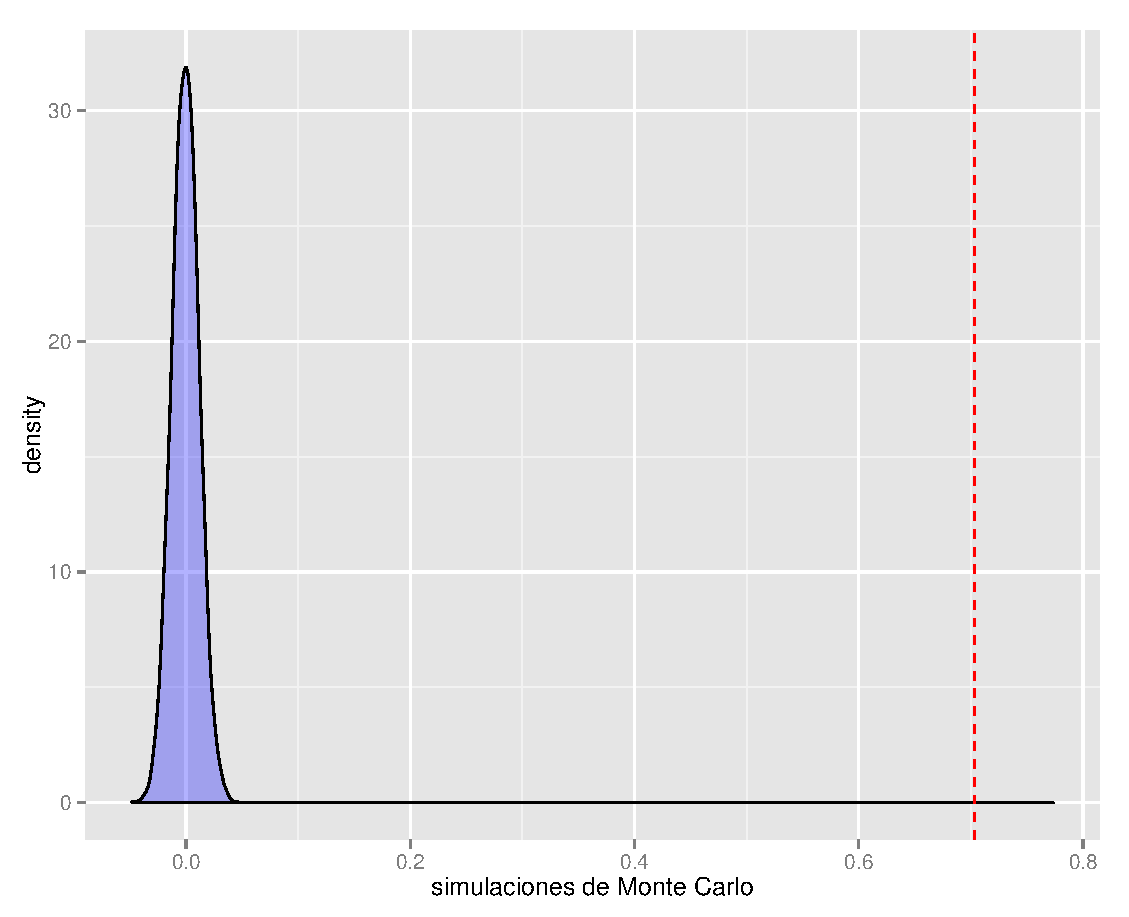
\includegraphics[width=.6\textwidth]{./plots/moran_density.pdf} \\
\caption{Densidad de la muestra de Monte Carlo de $\mathcal{I}$. La línea punteada índica donde se encuentra $\Hat{\mathcal{I}}$.}
\label{obj:morandensity}  
\end{figure}

\begin{itemize}
\item Viendo la forma de la densidad, el supuesto de normalidad parece muy razonable.  
\item Se observa como $\Hat{\mathcal{I}}$ cae muy lejos de la densidad de $I$ bajo el supuesto de no autocorrelación espacial. 
\end{itemize}



\subsection{Índice $\mathcal{C}$}
El valor del estimador $\Hat{\mathcal{C}}$, tiene el valor de 
\begin{equation}
\Hat{\mathcal{C}} = 0.2943260693 .
\end{equation}

Sea, $\mathcal{C}_0$ el valor esperado de $\mathcal{C}$ bajo la hipótesis nula, como esperamos autocorrelación espacial positiva para el índice de marginación, usamos la hipótesis alternativa $\mathcal{C}<\mathcal{C}_0$, sin embargo, como construimos el estadístico $z$ en la ecuación \ref{eq:zgeary}, esperamos que el estadístico $z$ observado sea significativamente mayor a $z$ bajo la hipótesis nula.


Así, utilizando los distintos supuestos, obtenemos los siguientes resultados.

\subsubsection{Bajo supuesto de normalidad}
Se obtuvieron los siguientes resultados
\begin{align*}
\EN [\widehat{\mathcal{C}}] =& 1,  \\ 
\VarN(\widehat{\mathcal{C}}) =& 0.0001911584, \\
z =& 51.0396, \\
\mbox{valor-p} <& 2.2 \times 10^{-16}.
\end{align*}

El valor del estadístico $z$ está muy lejos de la región de no rechazo de $H_0$, es claro que rechazamos la hipótesis nula de no autocorrelación, y por lo tanto, $\Hat{\mathcal{C}}$ es significativamente menor que $\mathcal{C}_0$.


\subsubsection{Bajo supuesto de aleatorización}

Bajo el supuesto de aleatorización, se obtuvieron resultados bastante similares

\begin{align*}
\widehat{\EN [\widehat{\mathcal{C}}]} =& 1,  \\ 
\widehat{\VarN(\widehat{\mathcal{C}})} =& 0.0001889559,  \\
z =& 51.3362, \\
\mbox{valor-p} <& 2.2 \times 10^{-16}.
\end{align*}

El valor del estadístico $z$ bajo este supuesto es practicamente el mismo que bajo el supuesto de normalidad, de la misma manera rechazamos la hipótesis nula de no autocorrelación espacial.
\subsubsection{Simulaciones de Monte Carlo}
Al igual que hicimos con el coeficiente de Morano, ahora muestreamos  de la distribución de $\mathcal{C}$. 

Usando $n_{sim}=9999$, se obtuvieron los siguientes resultados
\begin{align*}
\mbox{orden observado} &= 1,\\
\mbox{valor-p} &= 1\times 10^{-4}.
\end{align*}

Es decir, las  $9999$ observaciones del muestreo cayeron por encima de $\Hat{\mathcal{C}}$. Por lo tanto, esta prueba también nos indica claramente autocorrelación espacial positiva.

En la gráfica \ref{obj:gearydensity} podemos ver la densidad obtenida a partir de la muestra de Monte Carlo. 

\begin{figure}[!ht]
\centering
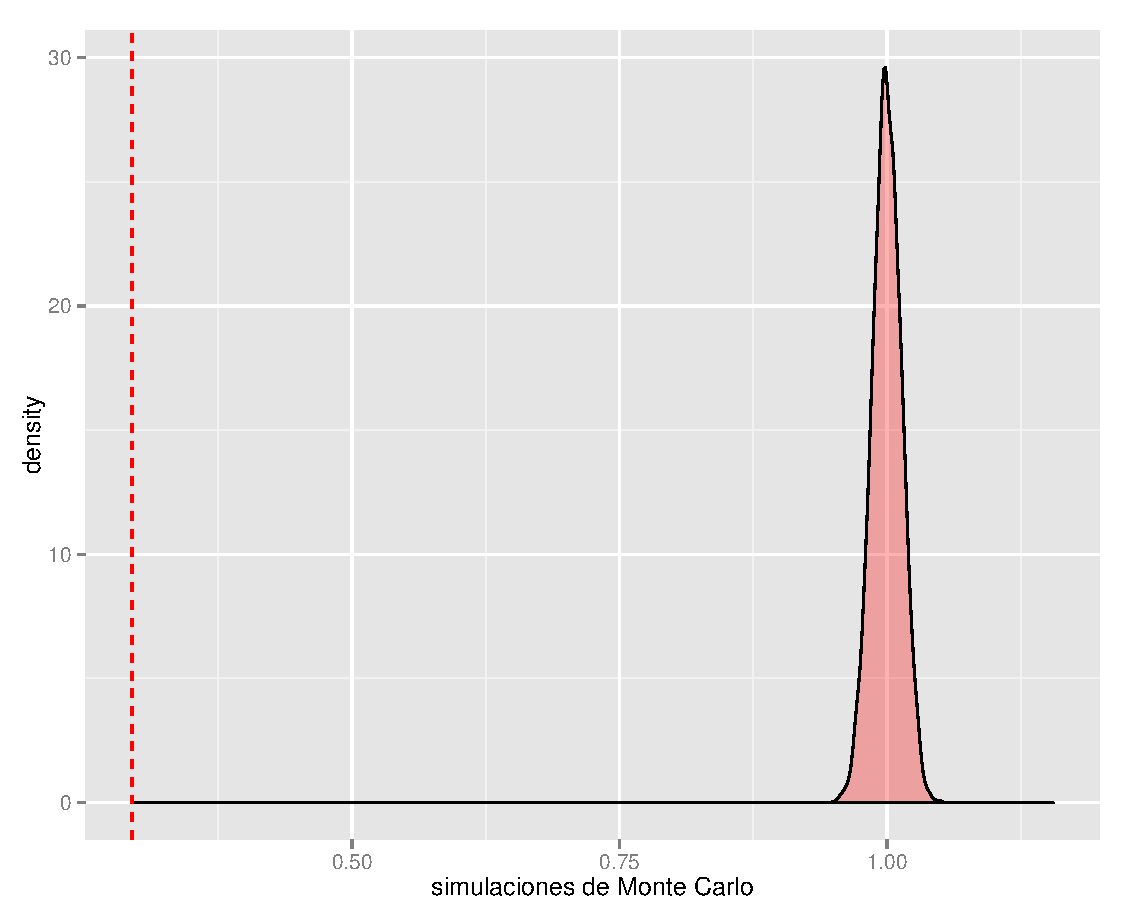
\includegraphics[width=.6\textwidth]{./plots/geary_density.pdf} \\
\caption{Densidad de la muestra de Monte Carlo de $\mathcal{C}$. La línea punteada índica donde se encuentra $\Hat{\mathcal{C}}$.}
\label{obj:gearydensity}  
\end{figure}

\begin{itemize}
\item Viendo la forma de la densidad, el supuesto de normalidad parece muy razonable.  
\item Se observa como $\Hat{\mathcal{C}}$ cae muy por debajo de la densidad de $C$ bajo el supuesto de no autocorrelación espacial. 
\end{itemize}




\section{Análisis de conglomerados}
Ahora, procedemos a agrupar los municipios por similitud. Para comparar los municipios, utilizaremos las variables que definen las cinco dimensiones de marginación propuesto por \citet{conapo04}: analf, sprim, sdren, selec, sagua, hacina, pisot, l5kha y bingreso.

Se utilizará el algoritmo de $k$-medias esférico que utiliza como medida de disimilitud entre observaciones, la disimilitud de cosenos.

\subsection{Determinación de $K^*$ utilizando el estadístico Gap}

Empezamos escogiendo el número de grupos $K^*$ a través del estadístico Gap. Escogiendo el número máximo de valores K a probar $M=10$, y $B=100$ para el tamaño de la muestra de Monte Carlo, podemos ver los resultados en la tabla~\ref{tab:gaptable}.

\begin{table}[ht]
\centering
\begin{tabular}{rrrrr}
  \hline
 & $\log{W_K}$ & $E^*\lbrace \log{W_K} \rbrace $ & $\mbox{Gap}_K$ & $s_K$ \\ 
  \hline
  1 & 5.5489 & 6.1259 & 0.5770 & 0.00389 \\ 
  2 & 5.3049 & 5.9731 & 0.6682 & 0.00318 \\ 
  3 & 5.1981 & 5.9205 & 0.7225 & 0.00298 \\ 
  4 & 5.1272 & 5.8754 & 0.7481 & 0.00305 \\ 
  5 & 5.0644 & 5.8431 & 0.7787 & 0.00283 \\ 
  6 & 5.0364 & 5.8140 & 0.7776 & 0.00307 \\ 
  7 & 5.0024 & 5.7921 & 0.7897 & 0.00307 \\ 
  8 & 4.9711 & 5.7707 & 0.7995 & 0.00290 \\ 
  9 & 4.9501 & 5.7543 & 0.8042 & 0.00293 \\ 
  10 & 4.9317 & 5.7392 & 0.8075 & 0.00300 \\ 
   \hline
\end{tabular}
\caption{Valor de Gap para $K$, $K=1,2, \dots, 10$. \label{tab:gaptable}}
\end{table}

Observando la gráfica \ref{obj:gapplot} y utilizando el criterio de \citet{hastie09} (véase la ecuación \ref{tibshiranicriteria}) encontramos que $K^*=5$.


\begin{figure}[!ht]
  \centering
  \caption{Gráfica del estadístico Gap. \label{obj:gapplot} }
  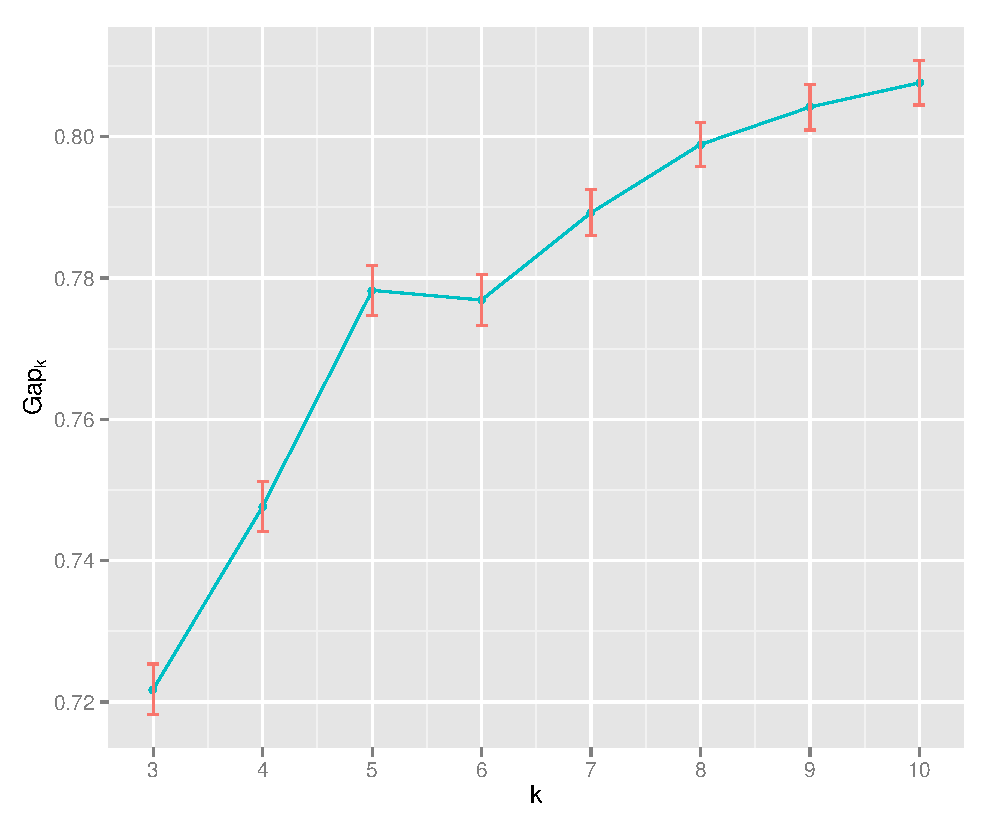
\includegraphics[width=.7\textwidth]{./plots/gap_plot.pdf}
\end{figure}

\subsection{Resultado de $K$-medias esféricas}
Habiendo obtenido que $K^*=5$, corremos el algoritmo de $k$-medias esféricas sobre las variables mencionadas anteriormente.

Podemos ver la distribución de  los 5 grupos en la tabla \ref{tabla5g} y en la gráfica \ref{obj:graf5g}.

\begin{table}[!ht]
\centering
\begin{tabular}{rrr}
  \hline
    & conteo & \% \\ 
  \hline
  1 & 490 & 20\% \\ 
  2 & 455 & 19\% \\ 
  3 & 808 & 33\% \\ 
  4 & 274 & 11\% \\ 
  5 & 429 & 17\% \\ 
   \hline
\end{tabular}
\caption{Tabla del tamaño de los 5 Grupos. \label{tabla5g}}
\end{table}

\begin{figure}[!ht]
  \centering
  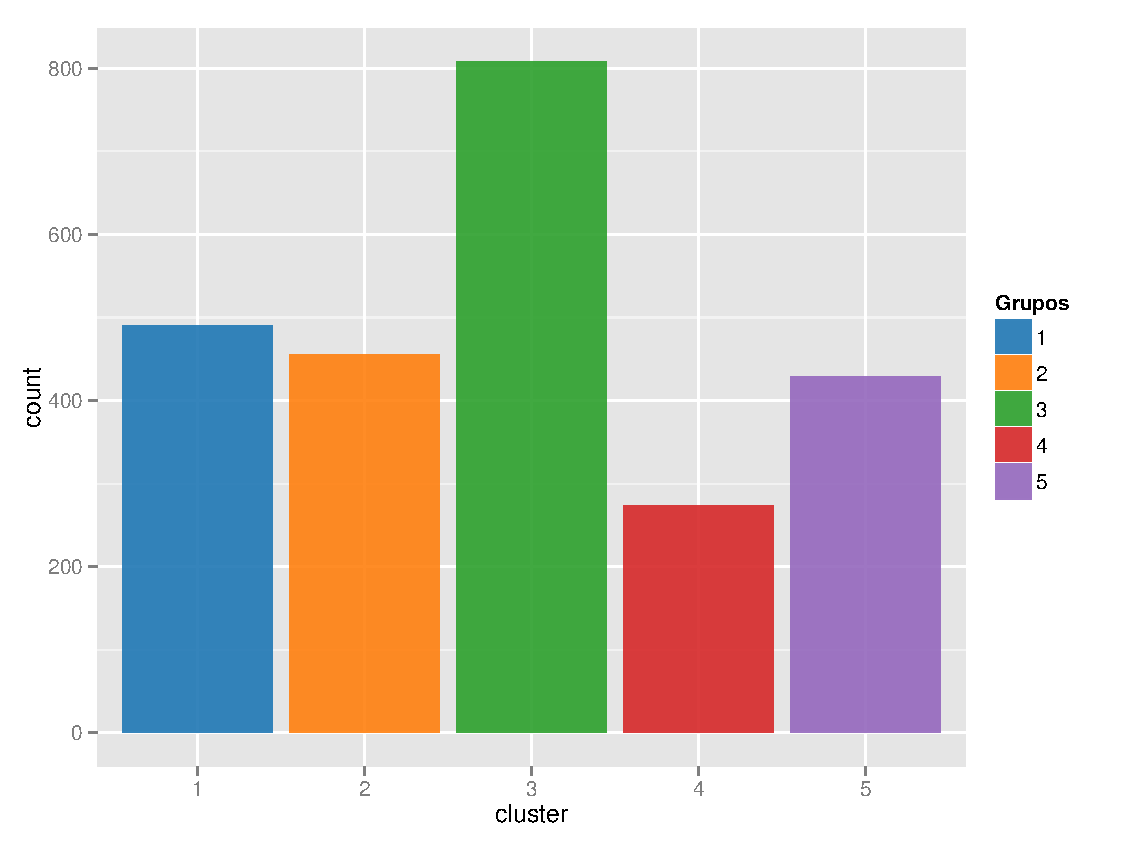
\includegraphics[width=.7\textwidth]{./plots/clustering_plot.pdf}
  \caption{Distribución de los grupos. \label{obj:graf5g} }
\end{figure}

Vemos que en el grupo 3 es donde cayeron más observaciones (33\%), mientras que en el 4 cayó el menor número de observaciones (11\%). Los demás grupos tienen una distribución similar.

Ahora, en la tabla \ref{tab:centroides} vemos los centroides de cada grupo. Éstos nos dan una caracterización de cada uno de los grupos.

\begin{table}
\centering
\begin{tabular}{rrrrrrrrrr}
  \hline
 & analf & sprim & sdren & selec & sagua & hacina & pisot & pl5khab & bingreso\\ 
  \hline
  1 & 0.07 & 0.24 & 0.05 & 0.02 & 0.05 & 0.30 & 0.05 & \textbf{0.81} & 0.44 \\ 
  2 & \textbf{0.14} & 0.29 & \textbf{0.08} & \textbf{0.06} & \textbf{0.32} & 0.37 & \textbf{0.15} & 0.60 & 0.51 \\ 
  3 & 0.13 & 0.30 & 0.05 & 0.03 & 0.07 & 0.37 & 0.12 & 0.66 & 0.54 \\ 
  4 & 0.09 & 0.30 & 0.03 & 0.02 & 0.09 & \textbf{0.67 }& 0.08 & 0.12 & \textbf{0.65} \\ 
  5 & 0.12 & \textbf{0.34} & 0.05 & 0.02 & 0.09 & 0.53 & 0.10 & 0.43 & 0.62 \\ 
   \hline
\end{tabular}
\caption{Centroides de los 5 conglomerados. \label{tab:centroides}}
\end{table}



En el mapa coroplético \ref{mapgroupsmarg} se colorea cada municipio de acuerdo al grupo en el que cayó.

\begin{landscape}
  \begin{figure}[!ht]
    \centering
    \caption[skip=0pt]{Mapa de México con los municipios coloreados por grupo. \label{mapgroupsmarg} }
    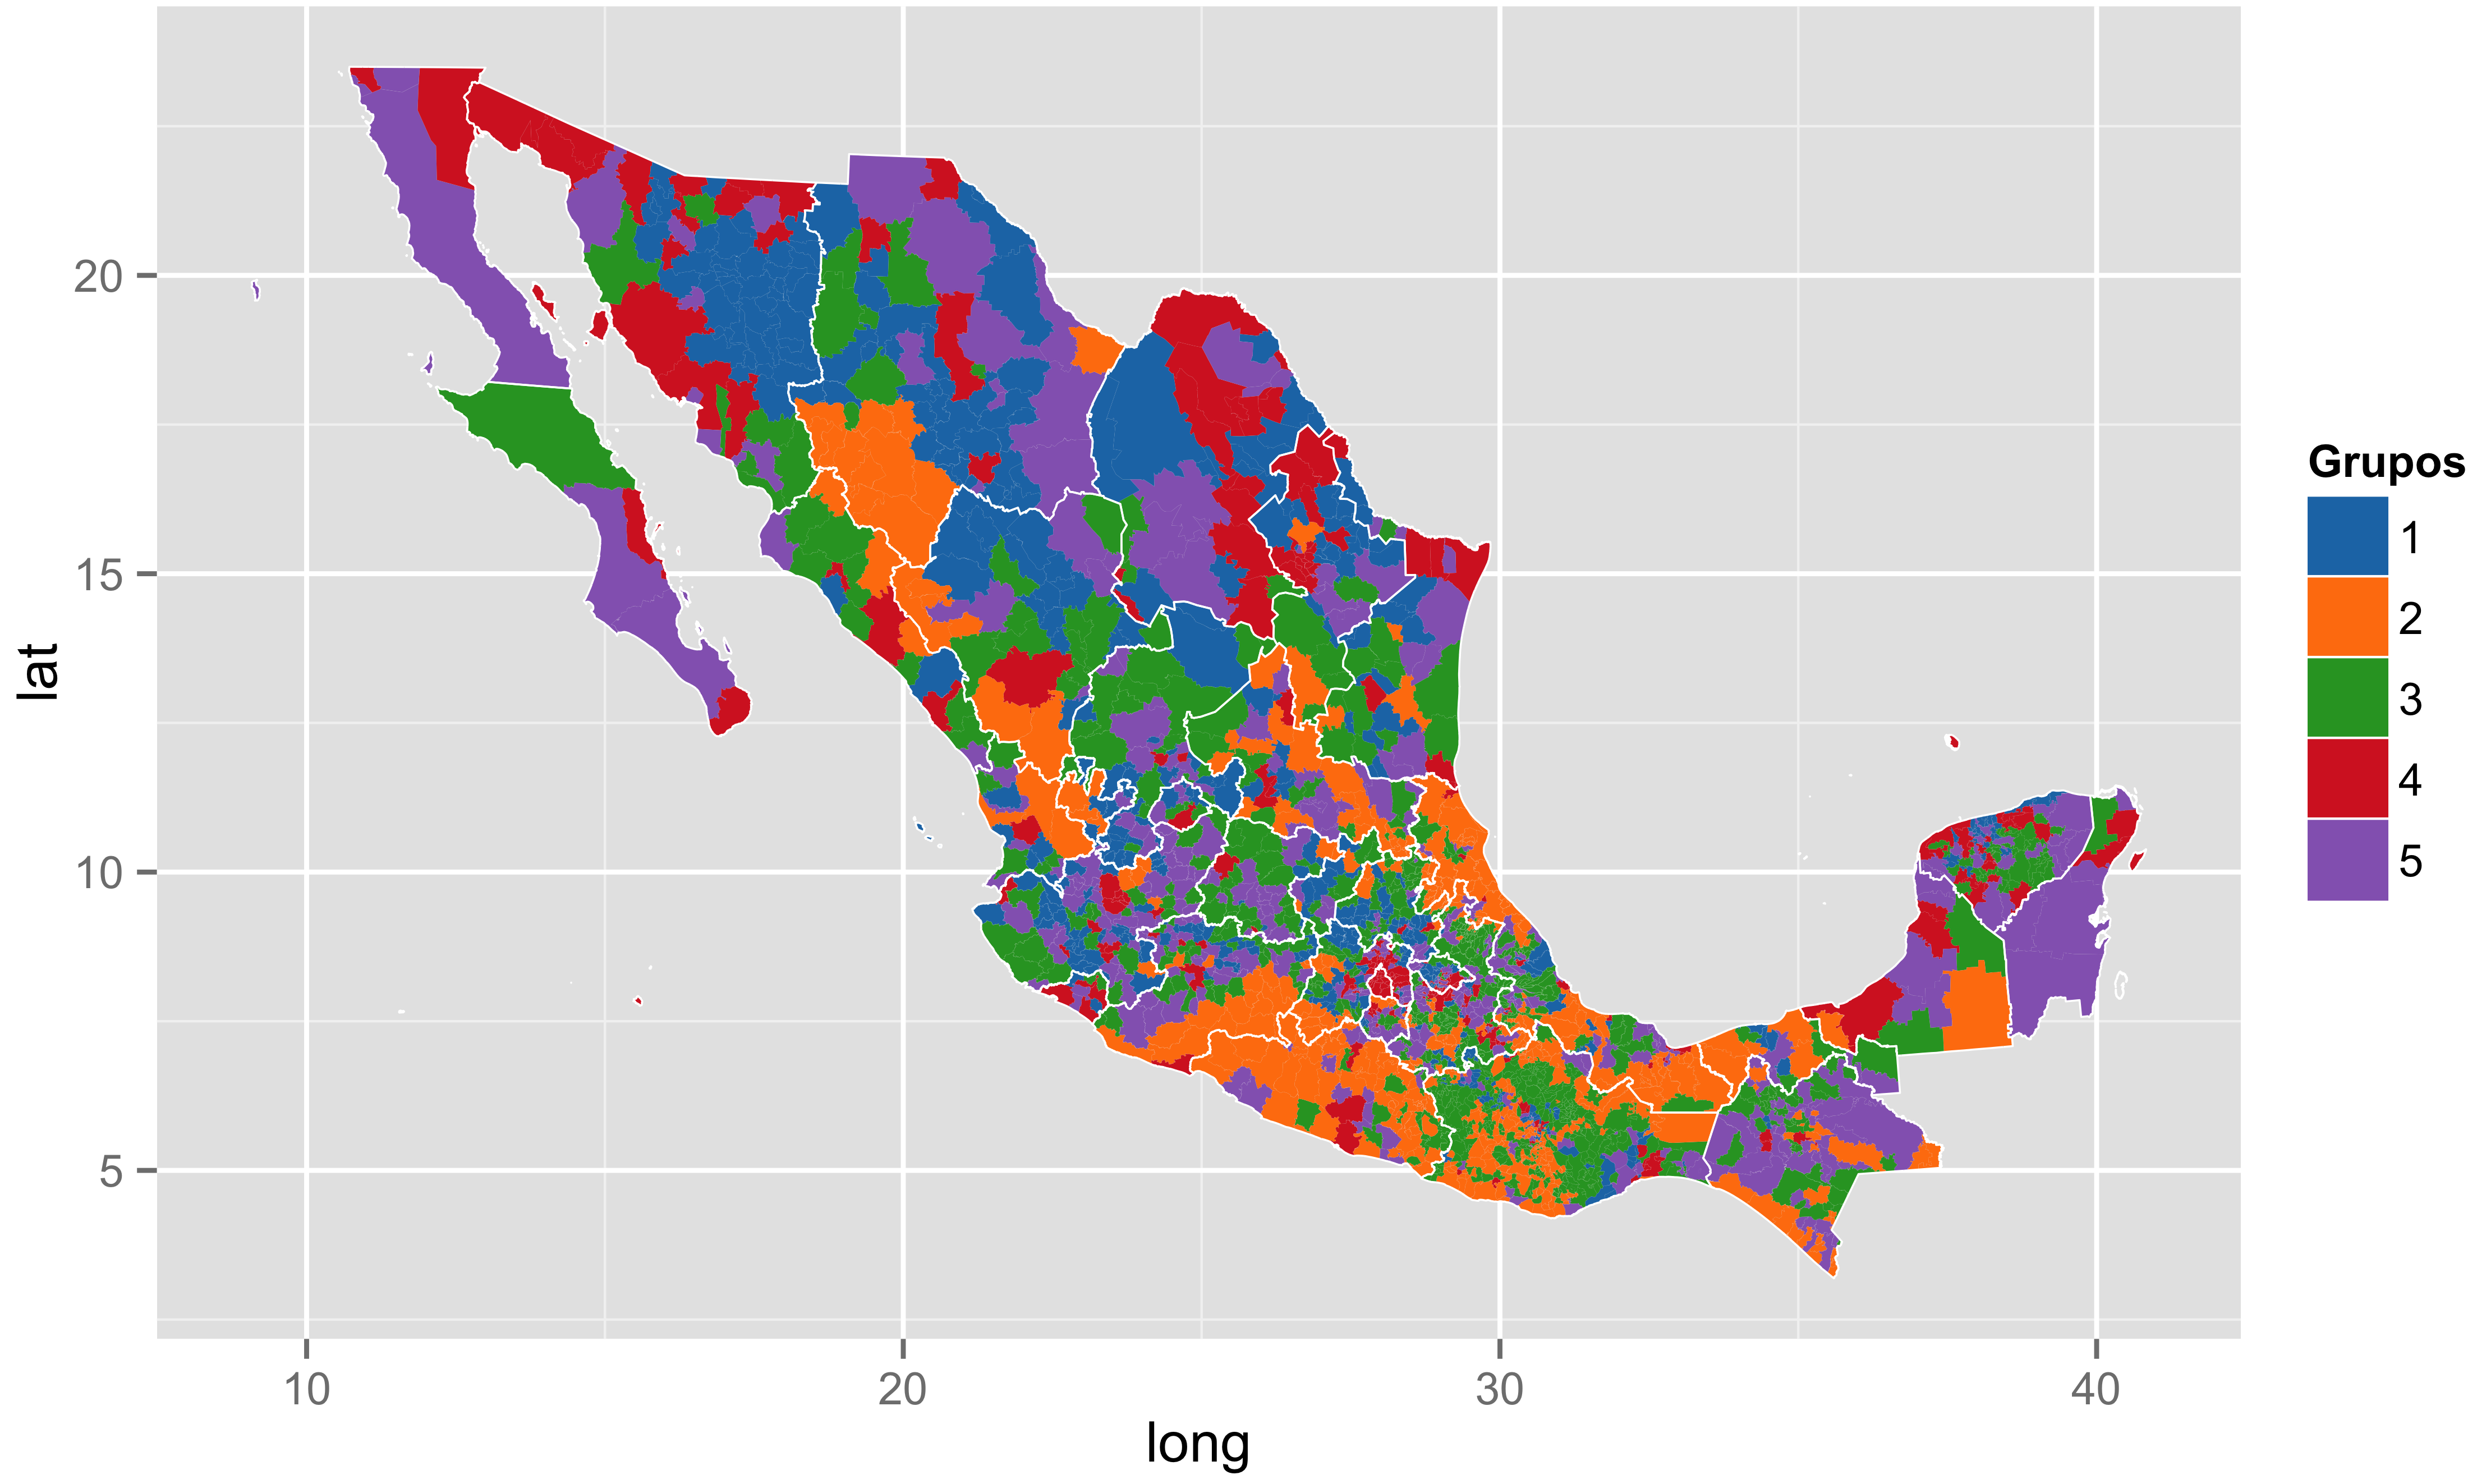
\includegraphics[width=1.4\textheight]{./maps/map5g.png}
  \end{figure}
\end{landscape}

En la gráfica \ref{obj:boxplotgroup} vemos la distribución por grupo de las 9 variables utilizadas en el algoritmo de conglomerados esféricos y en la gráfica \ref{obj:gradomarggrupos} vemos la distribución de los grupos de marginación por grupo.

\begin{figure}[!ht]
  \centering
  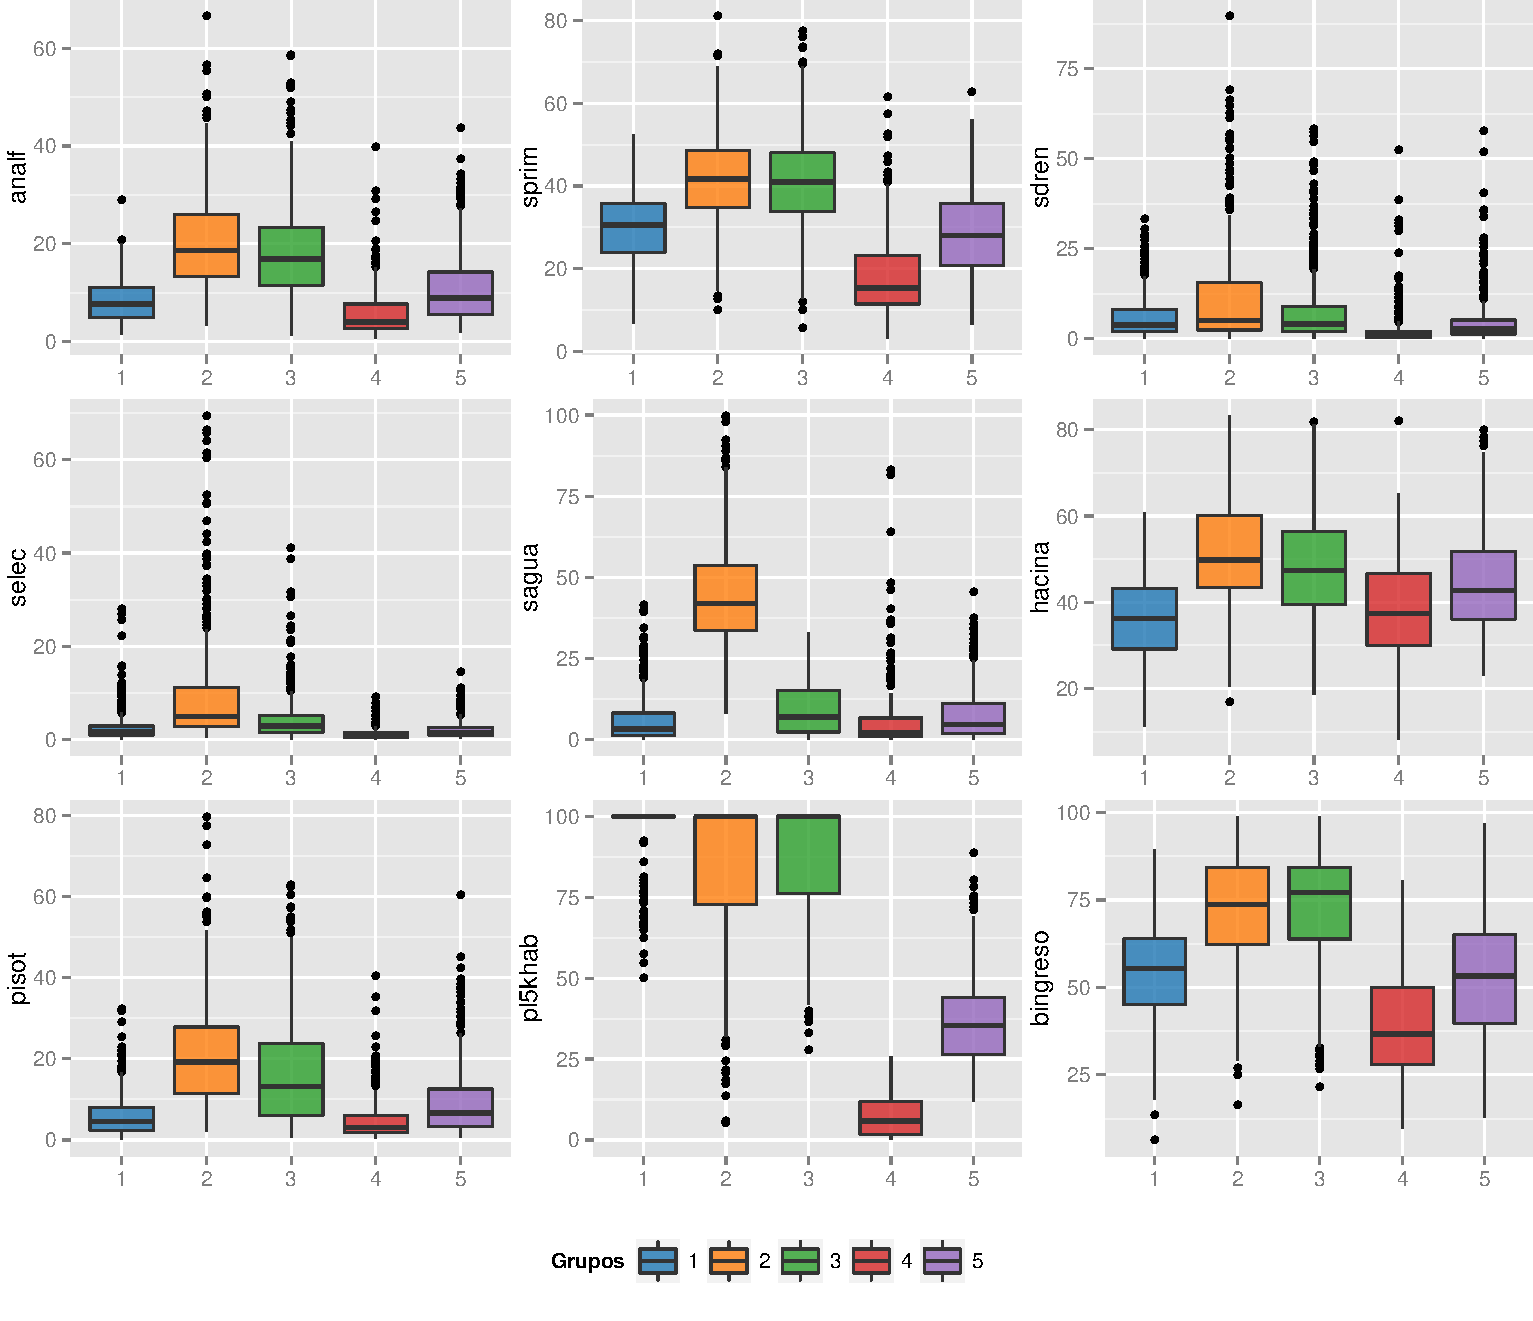
\includegraphics[width=\textwidth]{./plots/boxplot_bygroup.pdf}
  \caption{Distribución de variables de marginación por grupo. \label{obj:boxplotgroup} }
\end{figure}



\begin{figure}[!ht]
  \centering
  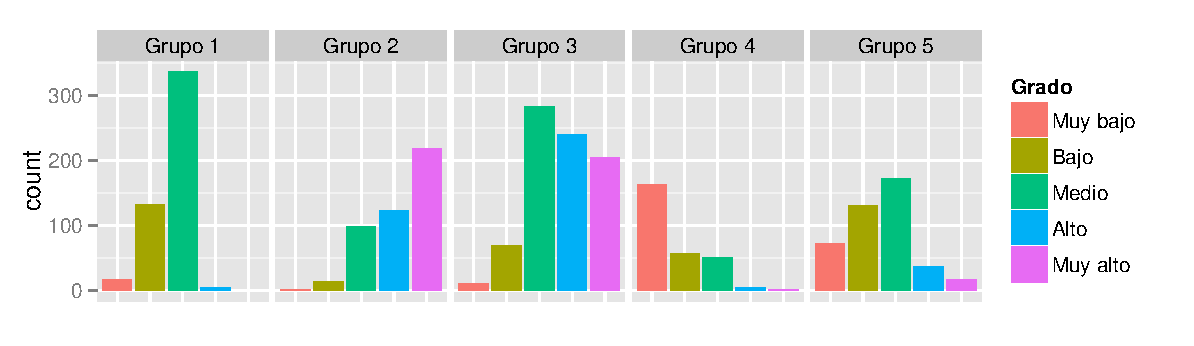
\includegraphics[width=\textwidth]{./plots/gmarg_group.pdf}
  \caption{Grado de marginación por grupo. \label{obj:gradomarggrupos} }
\end{figure}

A partir de la tabla \ref{tab:centroides}, las gráficas \ref{obj:gradomarggrupos} y \ref{obj:boxplotgroup} y observando el mapa \ref{mapgroupsmarg} podemos recalcar lo más característico de cada uno de los cinco grupos.

\begin{itemize}
\item \textbf{Grupo 1}: Se caracteriza por tener municipios con un alto porcentaje de población en localidades con menos de 5,000 habitantes y poco marginados. De hecho podemos observar en la gráfica \ref{obj:gradomarggrupos} que principalmente hay municipios con grado de marginación ``Medio'' y ``Medio Bajo''. Los municipios más cercanos al centroide los podemos ver en la tabla \ref{tab:grupo1}.

\begin{table}[!ht]
\centering
\begin{tabular}{rllrlr}
  \hline
 & nom\_mun & estado & imarges & gmarg & disim \\ 
  \hline
1 & Viesca & Coah & 21.74 & Medio & 0.00153 \\ 
  2 & San Gabriel & Jal & 22.51 & Medio & 0.00154 \\ 
  3 & Villa de la Paz & SLP & 20.62 & Medio & 0.00160 \\ 
  4 & Santa María del Oro & Nay & 23.24 & Medio & 0.00176 \\ 
  5 & Nazas & Dgo & 22.21 & Medio & 0.00206 \\ 
   \hline
\end{tabular}
\caption{Municipios más representativos del grupo 1. La columna disim corresponde a la disimilitud de cosenos entre la observación $i$ y el centroide del grupo 1. \label{tab:grupo1}}
\end{table}

\item \textbf{Grupo 2}: En este grupo se encuentran los municipios más marginados mencionados en la tabla \ref{tab:masmarg}. El grado de marginación de dichos municipios es ``Muy Alto'', ``Alto'' o ``Medio'' (ver gráfica \ref{obj:gradomarggrupos}). 
Se caracteriza por tener porcentajes altos en: población analfabeta y ocupantes en viviendas sin drenaje ni escusado, sin energía eléctrica, con piso de tierra y sin agua entubada. De hecho, es el grupo que tiene mayor porcentaje de viviendas sin agua entubada, siendo la principal característica que lo diferencia del grupo 3. Podemos ver en la tabla \ref{tab:grupo2} los municipios más representativos.

\begin{table}[ht]
\centering
\begin{tabular}{rllrlr}
  \hline
 & nom\_mun & estado & imarges & gmarg & disim \\ 
  \hline
1 & Xochiatipan & Hgo & 45.17 & Muy alto & 0.00216 \\ 
  2 & Coxquihui & Ver & 43.21 & Muy alto & 0.00356 \\ 
  3 & Playa Vicente & Ver & 32.72 & Alto & 0.00357 \\ 
  4 & Zozocolco de Hidalgo & Ver & 47.71 & Muy alto & 0.00372 \\ 
  5 & San Pedro Ixcatlán & Oax & 42.32 & Muy alto & 0.00416 \\ 
   \hline
\end{tabular}
\caption{Municipios más representativos del grupo 2. La columna disim corresponde a la disimilitud de cosenos entre la observación $i$ y el centroide del grupo 2. \label{tab:grupo2}}
\end{table}

\item \textbf{Grupo 3}: Como en el grupo 1, los municipios del grupo 3 tienen alto porcentaje de localidades pequeñas (menos de $5,000$ habitantes), pero los municipios tienen grado de marginación  ``Muy Alto'', ``Alto'' o ``Medio''. Además los municipios en este grupo, tienen porcetajes altos de población ocupada con ingreso de hasta 2 salarios mínimos. En la tabla \ref{tab:grupo3} podemos ver las observaciones más representativas.

\begin{table}[ht]
\centering
\begin{tabular}{rllrlr}
  \hline
 & nom\_mun & estado & imarges & gmarg & disim \\ 
  \hline
1 & Amatenango de la Frontera & Chis & 37.35 & Alto & 0.00102 \\ 
  2 & Coetzala & Ver & 35.01 & Alto & 0.00119 \\ 
  3 & Mártires de Tacubaya & Oax & 34.38 & Alto & 0.00160 \\ 
  4 & Totutla & Ver & 33.94 & Alto & 0.00187 \\ 
  5 & Juan N. Méndez & Pue & 36.20 & Alto & 0.00205 \\ 
   \hline
\end{tabular}
\caption{Municipios más representativos del grupo 3. La columna disim corresponde a la disimilitud de cosenos entre la observación $i$ y el centroide del grupo 3. \label{tab:grupo3}}
\end{table}

Es el grupo más grande con 808 municipios, representando un 33\% del total.

\item \textbf{Grupo 4}: En este grupo podemos encontrar muchos municipios con baja marginación. Es el grupo más pequeño con tan solo el 11\% de las observaciones. Todas las delegaciones del Distrito Federal y los principales municipios de la Ciudad de Monterrey, en Nuevo León, están en este grupo. En este grupo, los municipios tienen un porcentaje relativamente bajo de viviendas con algún nivel de hacinamiento, bajo porcentaje de población ocupada con ingreso de hasta 2 salarios mínimos y bajo porcentaje de población de 15 años o más sin primaria completa. Los cinco municipios más representativos los podemos ver en la tabla  \ref{tab:grupo4}.


\begin{table}[!ht]
\centering
\begin{tabular}{rllrlr}
  \hline
 & nom\_mun & estado & imarges & gmarg & disim \\ 
  \hline
1 & Jiutepec & Mor & 8.60 & Muy bajo & 0.00143 \\ 
  2 & Cuernavaca & Mor & 7.26 & Muy bajo & 0.00187 \\ 
  3 & Coatzacoalcos & Ver & 11.22 & Muy bajo & 0.00188 \\ 
  4 & Matamoros & Tam & 10.82 & Muy bajo & 0.00382 \\ 
  5 & Río Bravo & Tam & 13.51 & Muy bajo & 0.00392 \\ 
   \hline
\end{tabular}
\caption{Municipios más representativos del grupo 4. La columna disim corresponde a la disimilitud de cosenos entre la observación $i$ y el centroide del grupo 4. \label{tab:grupo4}}
\end{table}

Podemos encontrar también algunos lugares turísticos como San Cristóbal de las Casas, Acapulco, Benito Juárez en Quintana Roo (aquí se encuentra Cancún), Los Cabos, Puerto Vallarta, Veracruz, etc.

\item \textbf{Grupo 5}: Este grupo es muy parecido al grupo 1, pero los municipios dentro del grupo 5 tienen mayor porcentaje de poblaciones con más de $5,000$ habitantes, es decir, tienen poblaciones más grandes. Los cinco municipios más cerca del centroide 5 se encuentran en la tabla \ref{tab:grupo5}.

\begin{table}[ht]
\centering
\begin{tabular}{rllrlr}
  \hline
 & nom\_mun & estado & imarges & gmarg & disim \\ 
  \hline
1 & Villagrán & Gto & 16.83 & Bajo & 0.00137 \\ 
  2 & Cortazar & Gto & 16.38 & Bajo & 0.00186 \\ 
  3 & Angel Albino Corzo & Chis & 35.21 & Alto & 0.00232 \\ 
  4 & San Juan Bautista Tuxtepec & Oax & 19.51 & Bajo & 0.00277 \\ 
  5 & Celaya & Gto & 11.76 & Muy bajo & 0.00294 \\ 
   \hline
\end{tabular}
\caption{Municipios más representativos del grupo 5. La columna disim corresponde a la disimilitud de cosenos entre la observación $i$ y el centroide del grupo 5. \label{tab:grupo5}}
\end{table}

\end{itemize}

Otro punto que podemos destacar observando el mapa \ref{mapgroupsmarg}, es que existe cierta uniformidad espacial entre miembros del mismo grupo. Es decir, vemos que regiones que pertenecen al mismo grupo, comparten frontera. 

En la próxima sección se harán las pruebas de hipótesis para detectar la presencia de autocorrelación espacial positiva.


\section{Prueba de conteo de fronteras para conglomerados}

Sean $\Hat{N_{rs}}$ los conteo observado,  $N_{rs,0}$ los conteo esperado de fronteras del tipo $rs$, $r,s=1,2,3,4,5$.

Dado que no contamos con las $p_i$'s (probabilidad de que una región sea de tipo $i$) a priori, las estimamos a partir de los datos. Por lo tanto, en el siguiente análisis de autocorrelación espacial se utilizará el supuesto de muestreo sin reemplazo. También se utilizarán los pesos binarios estandarizados por renglón.

La tabla \ref{tab:conteobordes} donde se muestran los conteos de fronteras observados conteos esperados y las varianzas bajo muestreo sin reemplazo y el valor $z$ calculado. 
\begin{table}[ht]
\centering
\begin{tabular}{rrrrr}
  \hline
 & $\Hat{N_{rs}}$  & $N_{rs,0}$ & $\Var$ & $z$ \\ 
  \hline
  1:1 & 98.61 & 48.80 & 6.53 & 19.49 \\ 
  2:2 & 110.35 & 42.07 & 5.77 & 28.43 \\ 
  3:3 & 194.99 & 132.80 & 14.00 & 16.62 \\ 
  4:4 & 50.36 & 15.23 & 2.36 & 22.88 \\ 
  5:5 & 63.59 & 37.40 & 5.22 & 11.46 \\ 
  2:1 & 35.95 & 90.81 & 12.56 & -15.48 \\ 
  3:1 & 103.48 & 161.27 & 20.00 & -12.92 \\ 
  3:2 & 138.83 & 149.75 & 18.74 & -2.52 \\ 
  4:1 & 48.76 & 54.69 & 7.96 & -2.10 \\ 
  4:2 & 18.10 & 50.78 & 7.48 & -11.95 \\ 
  4:3 & 42.67 & 90.18 & 11.81 & -13.82 \\ 
  5:1 & 82.05 & 85.63 & 11.93 & -1.03 \\ 
  5:2 & 55.61 & 79.51 & 11.19 & -7.14 \\ 
  5:3 & 122.55 & 141.19 & 17.79 & -4.42 \\ 
  5:4 & 62.10 & 47.88 & 7.11 & 5.33 \\ 
  Jtot & 710.10 & 951.70 & 37.24 & -39.59 \\ 
   \hline
\end{tabular}
\caption{Conteo de fronteras.}
\label{tab:conteobordes}
\end{table}

Los conteos de fronteras entre municipios del mismo color son mucho mayores que lo esperado.Viendo el valor $z$ entre las fronteras del tipo $rr$, podemos resaltar que, para $1:1$, es el más alto con $28.43$; mientras que para $5:5$, es el más bajo. Esto indica que 
que las regiones del grupo $1$ están más aglomeradas que las regiones del grupo $5$ (ver mapa \ref{mapgroupsmarg}. 

Otro punto a mencionar es el caso del conteo $N_{54}$, es el único conteo de fronteras de tipo $rs$ con $r\neq s$, cuyo valor $z$ es positivo. Es decir, el número de fronteras entre regiones del grupo $4$ y $5$ es mayor a esperado. Podemos corroborarlo en el mapa \ref{mapgroupsmarg}, muchos municipios rojos tienen frontera con morados.

Como ejemplo de no autocorrelación espacial, se presenta el mapa \ref{fig:rmap_5g_ej}, donde las etiquetas de los grupos están permutadas de manera aleatoria. 

\begin{figure}[!ht]
  \centering
  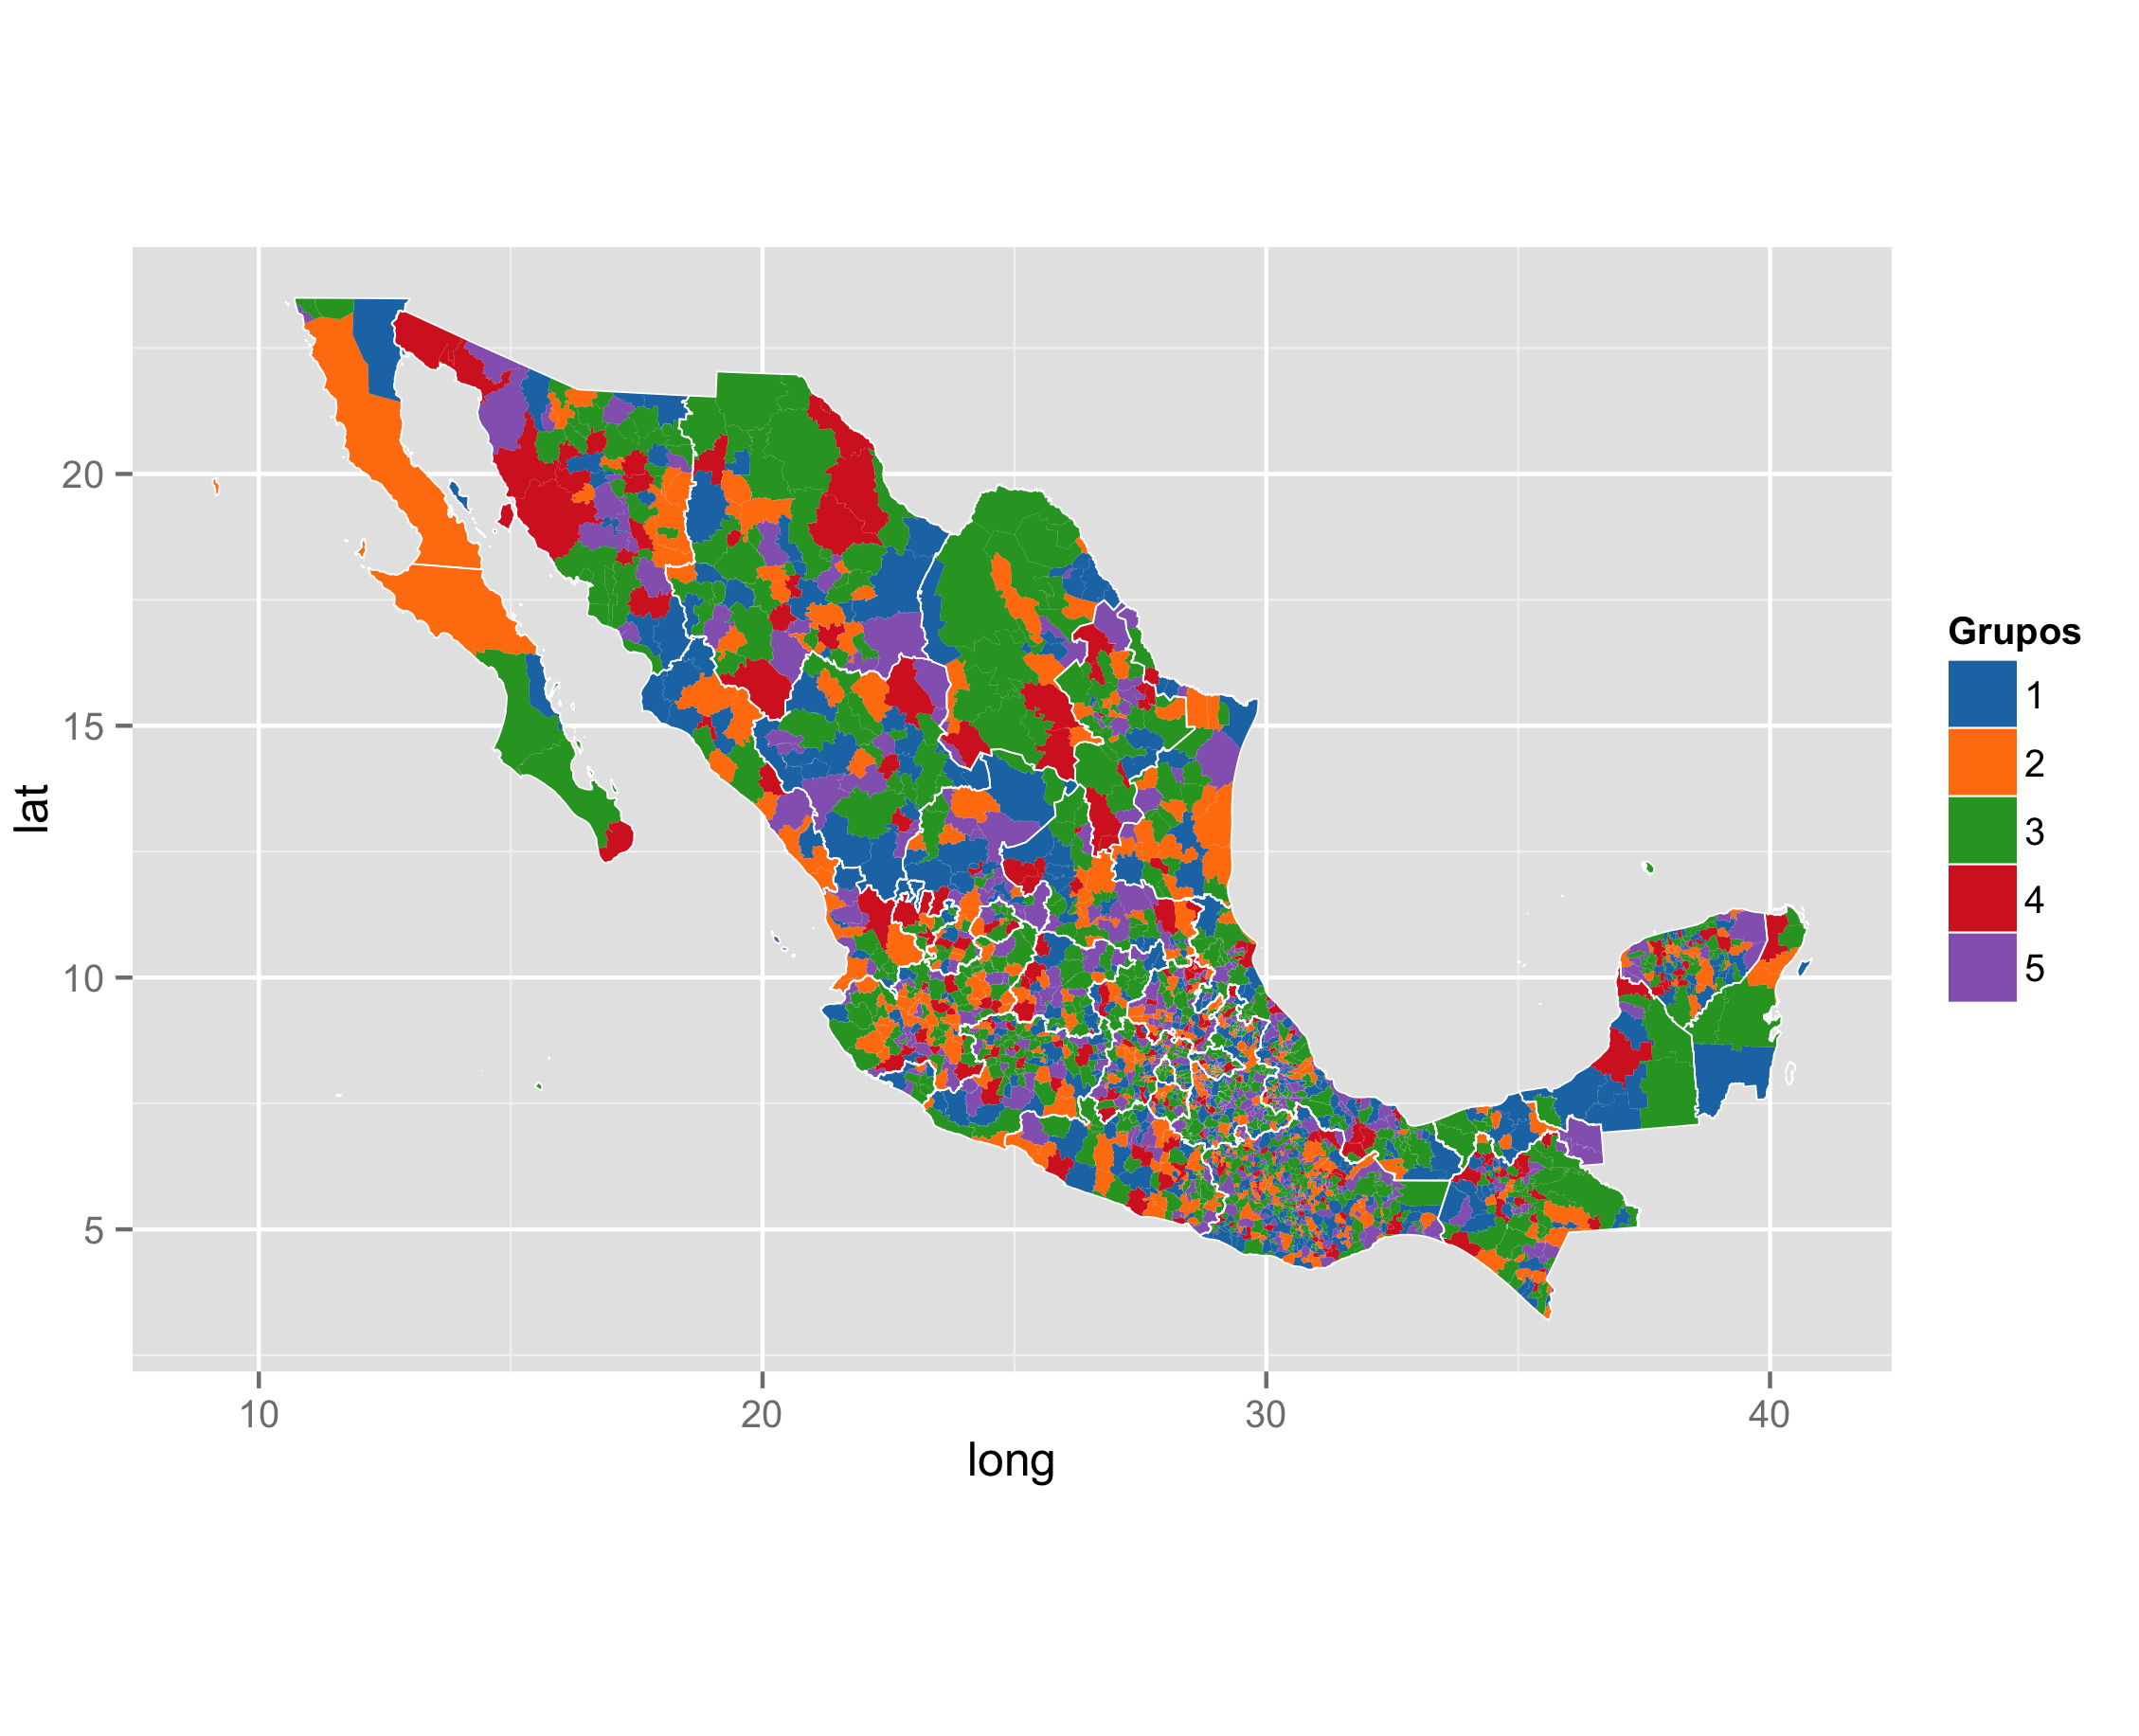
\includegraphics[width=\textwidth]{./maps/rmap5g.png} \\
  \caption{ Permutación aleatoria de los grupos obtenidos mediante el algoritmo de $k$-medias esféricas.}
  \label{fig:rmap_5g_ej}  
\end{figure}
Ahora, corroboramos lo dicho haciendo pruebas de hipótesis sobre $N_{rr}$ , $r=1, 2, 3, 4, 5$.

\subsubsection{Bajo supuesto de normalidad}
Suponiendo que $N_{11}, N_{22}, \dots, N_{55}$ se distribuyen normal, la tabla \ref{tab:conteobordesprueba} muestra la misma información que la tabla \ref{tab:conteobordes} para conteo de bordes del mismo tipo, pero se añade el valor $p$ porque ya estamos suponiendo una distribución.

\begin{table}[ht]
\centering
\begin{tabular}{rrrrrr}
  \hline
  grupo & $\Hat{N_{rs}}$  & $N_{rs,0}$ & $\Var$ & $z$ & valor-p \\ 
  \hline
  1 & 98.61 & 48.80 & 6.53 & 19.49 & $< 2.2 \times 10^{-16}$ \\ 
  2 & 110.35 & 42.07 & 5.77  & 28.43 & $< 2.2 \times 10^{-16}$ \\ 
  3 & 194.99 & 132.80 & 14.00 & 16.62 & $< 2.2 \times 10^{-16}$ \\ 
  4 & 50.36 & 15.23 & 2.36 & 22.88 & $< 2.2 \times 10^{-16}$ \\ 
  5 & 63.59 & 37.40 & 5.22 & 11.46 & $< 2.2 \times 10^{-16}$ \\ 
   \hline
\end{tabular}
\caption{Pruebas de hipótesis para $N_{rr}$ , $r=1, 2, 3, 4, 5$.}
\label{tab:conteobordesprueba}
\end{table}

Ahora, interpretando el valor $z$ bajo el supuesto de normalidad, los conteos $\Hat{N_{rs}}$'s caen muy lejos de la región de no rechazo. Por lo tanto, rechazamos la hipótesis nula de no autocorrelación espacial.


\subsubsection{Simulaciones de Monte Carlo}
Ahora, realizamos la prueba omitiendo el supuesto de normalidad. Sean $N_{rs,0}^*$ y $\Var^*$ el valor esperado y la varianza esperada, ambos calculados a partir de la muestra de Monte Carlo. Usando una muestra de tamaño $n_{sim}=9999$, podemos ver los resultados en la tabla \ref{tab:joincountsmontecarlo}.

% latex table generated in R 3.0.2 by xtable 1.7-3 package
% Thu Oct 30 11:32:06 2014
\begin{table}[!ht]
\centering
\begin{tabular}{rrrrrr}
  \hline
 grupo & $\Hat{N_{rs}}$  & $N_{rs,0}^*$ & $\Var^*$ & orden & valor-p \\ 
  \hline
  1 & 98.61 & 48.82 & 6.44 & 10000 & $1\times 10^{-4}$ \\ 
  2 & 110.35 & 42.11 & 5.92 & 10000 & $1\times 10^{-4}$ \\ 
  3 & 194.99 & 132.86 & 13.68 & 10000 & $1\times 10^{-4}$ \\ 
  4 & 50.36 & 15.23 & 2.34 & 10000 & $1\times 10^{-4}$ \\ 
  5 & 63.59 & 37.37 & 5.26 & 10000 & $1\times 10^{-4}$ \\ 
   \hline
\end{tabular}
\caption{Resultados de simulaciones de Monte Carlo.}
\label{tab:joincountsmontecarlo}
\end{table}

El conteo $\Hat{N_{rr}}$ es mayor que las $9,999$ simulaciones de Monte Carlo , para $r=1,2,3,4,5$. Es decir, para todos los grupos, se rechaza la hipótesis nula de no autocorrelación. Podemos ver la distribución de las muestras simuladas y donde caen los valores observados en la gráfica \ref{obj:jcdensity}.

\begin{figure}[!ht]
  \centering
  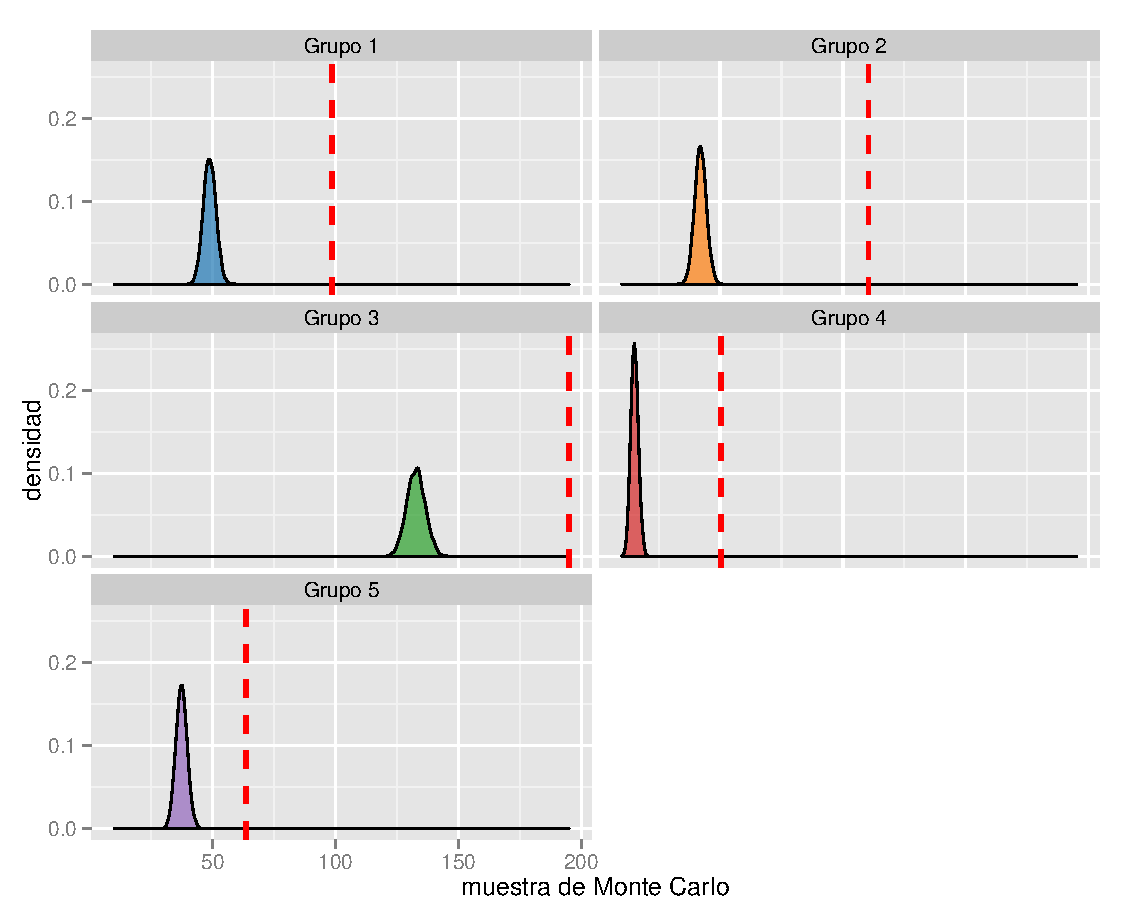
\includegraphics[width=\textwidth]{./plots/jc_density.pdf}
  \caption{Densidad de la muestra de Monte Carlo de $N_{rr}$. La línea punteada índica donde se encuentra $\Hat{N_{rr}}$. \label{obj:jcdensity} }
\end{figure}
